% ============================================================================
% TUGAS AKHIR (TA 2) — Program Studi Statistika UGM
% VERSI ANALISIS PENUH — disusun sebagai satu berkas mandiri.
%
% Berbeda dari `skripsi_ta2.tex` yang memanggil bab/*.tex, berkas ini memuat
% seluruh naskahnya sendiri supaya dapat dibaca berurutan sebagai satu
% argumen utuh: dari rumusan masalah, penurunan matematis, rancangan
% eksperimen, sampai bukti berjenjang dan batasannya.
%
% Pasar yang dipakai: Bursa Efek Indonesia, indeks LQ45, 2021--2025.
% Kompilasi: latexmk -pdf skripsi_v_claude.tex
% ============================================================================
\documentclass{laporanta1statugm}

\usepackage{bm}
\usepackage{booktabs}
\usepackage{longtable}
\usepackage[most]{tcolorbox}

\definecolor{kartubiru}{RGB}{31,56,100}
\definecolor{kartuabu}{RGB}{247,247,249}
\definecolor{kartubadge}{RGB}{214,232,255}

\newtcolorbox{kartufaktor}[1]{
  enhanced, breakable,
  colback=white, colframe=kartubiru,
  boxrule=0.9pt, arc=2.5mm,
  title={\bfseries #1}, fonttitle=\large,
  coltitle=white, colbacktitle=kartubiru,
  attach boxed title to top left={xshift=0mm, yshift=-2.8mm},
  boxed title style={arc=2mm, boxrule=0pt, left=3mm, right=3mm},
  top=5mm, left=4mm, right=4mm, bottom=3mm
}
\newtcolorbox{kotakekspresi}{
  colback=kartuabu, colframe=black!25,
  boxrule=0.5pt, arc=1.5mm,
  left=2mm, right=2mm, top=1.5mm, bottom=1.5mm,
  fontupper=\ttfamily\small
}
\newcommand{\barisfield}[2]{\makebox[3.8cm][l]{\textbf{#1}}#2\par\vspace{0.8mm}}
\newcommand{\code}[1]{\texttt{#1}}

\titleind{Evaluasi Formulasi Langkah Laten pada Komunikasi Sistem Multi-Agen:
Disosiasi antara Validitas Keluaran dan Mutu Sinyal pada Penalaran Umum dan
Pembangkitan Faktor Simbolik}

\fullname{Harun Yahya}
\NIM{22/505239/PA/21749}
\yearsubmit{2026}

\begin{document}
\cover

\newpage\phantomsection\addcontentsline{toc}{chapter}{DAFTAR ISI}
\tableofcontents

% ===========================================================================
\pagenumbering{arabic}\setcounter{page}{1}
\chapter{PENDAHULUAN}

\section{Latar Belakang}

Model bahasa besar (\textit{large language model}, LLM) semakin sering
dijalankan bukan sebagai model tunggal, melainkan sebagai sistem
\textit{multi-agent}: beberapa salinan model diberi peran berbeda dan bekerja
berurutan, saling meneruskan hasil pekerjaan sampai jawaban akhir terbentuk
\citep{russellnorvig}. Pembagian peran semacam itu memperbaiki mutu jawaban
pada tugas yang menuntut perencanaan dan perbaikan bertahap.

Pada hampir seluruh sistem tersebut, medium penghubung antar-agen adalah teks.
Setiap agen mengubah penalaran internalnya menjadi untaian token, lalu agen
berikutnya menguraikan untaian itu kembali menjadi representasi internalnya
sendiri. Proses bolak-balik ini menimbulkan dua persoalan. Pertama, biaya
komputasi meningkat karena setiap penyerahan pekerjaan mengharuskan
pembangkitan token yang panjang. Kedua, terjadi penyempitan kanal: representasi
internal yang kaya dimampatkan menjadi barisan simbol diskret, dan hanya
sebagian yang dapat dipulihkan agen penerima \citep{latentmas, cache2cache}.

Sebagai jawaban, \citet{latentmas} mengusulkan LatentMAS, kerangka kolaborasi
\textit{multi-agent} yang berlangsung sepenuhnya di ruang laten. Alih-alih
bertukar teks, tiap agen menjalankan sejumlah langkah penalaran di ruang
representasi kontinu, lalu menyerahkan memori kerjanya berupa
\textit{key-value cache} dari mekanisme \textit{attention} \citep{vaswani}
kepada agen berikutnya. Pendekatan ini bagian dari paradigma penalaran laten
yang lebih luas \citep{coconut, latentsurvey}.

Inti teknis LatentMAS adalah satu persamaan. Sebuah \textit{hidden state}
$\bm{h}$ yang dihasilkan lapisan terakhir transformer hidup di ruang keluaran,
yaitu ruang yang dibaca kepala bahasa untuk menghasilkan \textit{logit};
sedangkan masukan yang diharapkan lapisan pertama adalah \textit{embedding}
token, yang hidup di ruang masukan. Kedua ruang berdimensi sama tetapi tidak
sama. LatentMAS menjembataninya dengan sebuah matriks $\bm{M}$ hasil regresi
ridge \citep{ridge} yang dipasang sekali di awal, lalu memakai $\bm{h}\bm{M}$
sebagai masukan langkah berikutnya.

Penelitian pendahuluan pada penelitian ini menemukan bahwa persamaan tersebut
gagal total ketika muatan yang harus dibawa kanal laten bersifat
\textit{simbolik} --- nama fungsi, pengenal, ekspresi --- dengan
\textit{recall} 0,000 mutlak, sementara empat formulasi alternatif yang
memproyeksikan langkah laten kembali ke \textit{convex hull} embedding token
nyata seluruhnya mendarat pada 0,34--0,38. Temuan itu menimbulkan pertanyaan
yang menjadi pokok skripsi ini: apakah keunggulan keluarga formulasi
alternatif tersebut bersifat umum, ataukah spesifik untuk muatan simbolik?

Untuk menjawabnya, dua kategori tugas dievaluasi berdampingan dengan
perlakuan setara: \textit{penalaran umum} (tiga tolok ukur baku) dan
\textit{pembangkitan faktor simbolik} (ekspresi \textit{alpha} atas data pasar
saham). Kategori kedua memakai data Bursa Efek Indonesia, indeks LQ45, periode
2021--2025.

\section{Rumusan Masalah}

\begin{enumerate}
  \item Bagaimana kelima formulasi langkah laten diturunkan dari satu bentuk
        umum, dan sifat geometris apa yang membedakan formulasi resmi LatentMAS
        dari keluarga relaksasi diskret?
  \item Apakah keluarga relaksasi diskret menghasilkan keluaran yang lebih
        \textit{valid} dibanding formulasi resmi LatentMAS, dan seberapa besar
        efeknya?
  \item Apakah keunggulan itu juga terjadi pada \textit{mutu sinyal} keluaran,
        yaitu daya prediksi faktor yang dihasilkan terhadap imbal hasil saham?
  \item Berapa besar penghematan biaya komputasi kanal laten murni dibanding
        kanal teks penuh, dan apakah penghematan itu menurunkan mutu keluaran?
  \item Bagaimana bentuk hubungan antara kedekatan geometris representasi laten
        terhadap ruang embedding dan kinerja hilirnya --- monoton, berambang,
        atau tidak berpola?
\end{enumerate}

\section{Tujuan Penelitian}

\begin{enumerate}
  \item Menurunkan kelima formulasi langkah laten dari satu bentuk umum dan
        menetapkan kriteria geometris yang memisahkan keduanya.
  \item Menguji secara formal perbedaan validitas keluaran antara keluarga
        relaksasi diskret dan formulasi resmi LatentMAS pada dua medium
        komunikasi.
  \item Menguji apakah perbedaan validitas itu diikuti perbedaan mutu sinyal,
        diukur dengan \textit{rank information coefficient} pada data LQ45.
  \item Mengukur biaya komputasi tiap medium dengan denominator yang seragam.
  \item Memetakan bentuk hubungan geometri--kinerja melalui sumbu interpolasi
        kontinu antara dua formulasi ujung.
\end{enumerate}

\section{Manfaat Penelitian}

Secara teoretis, penelitian ini memberi kriteria geometris yang dapat diuji
untuk menilai formulasi langkah laten mana pun, serta bukti empiris bahwa
kriteria itu memisahkan kinerja secara tajam. Secara praktis, penelitian ini
menunjukkan bahwa komunikasi antar-agen lewat \textit{key-value cache} dapat
memangkas biaya token secara besar tanpa menurunkan keandalan keluaran, asalkan
formulasi langkah latennya dipilih dengan benar.

\section{Batasan Penelitian}

\begin{enumerate}
  \item Model tunggal, \code{Qwen3-8B} \citep{qwen3}, tanpa pelatihan ulang.
        Seluruh formulasi bersifat \textit{training-free}.
  \item Rantai agen bersifat \textit{single-pass}: proposal $\to$ innovate
        $\to$ construct, tanpa loop evolusi.
  \item Universe pasar dibatasi pada 37 konstituen LQ45 yang memiliki data
        lengkap; implikasinya dibahas pada Subbab 3.7 dan 5.3.
  \item Metrik portofolio bersifat deskriptif; kesimpulan antar-formulasi
        disandarkan pada koefisien informasi yang memiliki uji hipotesis.
  \item Penelitian ini tidak mengklaim menemukan strategi perdagangan yang
        menguntungkan.
\end{enumerate}

% ===========================================================================
\chapter{TINJAUAN PUSTAKA DAN LANDASAN TEORI}

\section{Transformer dan Dua Ruang Representasi}

Sebuah transformer \textit{decoder-only} \citep{vaswani} memetakan barisan
token menjadi barisan \textit{hidden state}. Pada posisi terakhir, keluaran
lapisan terakhir dinotasikan $\bm{h}\in\mathbb{R}^{d}$. Untuk \code{Qwen3-8B},
$d = 4096$ dan ukuran kosakata $V = 151\,936$.

Model memiliki dua matriks embedding yang berbeda:
\[
  \bm{W}_{\text{in}}\in\mathbb{R}^{V\times d}, \qquad
  \bm{W}_{\text{out}}\in\mathbb{R}^{V\times d}.
\]
Baris ke-$i$ dari $\bm{W}_{\text{in}}$ adalah representasi token $i$ sebagai
\emph{masukan}; baris ke-$i$ dari $\bm{W}_{\text{out}}$ adalah arah pada ruang
keluaran yang memilih token $i$. \textit{Logit} untuk token berikutnya adalah
\begin{equation}
  \bm{\ell} = \bm{W}_{\text{out}}\,\bm{h}, \qquad
  \ell_i = \langle \bm{W}_{\text{out}}[i], \bm{h}\rangle .
  \label{eq:logit}
\end{equation}

Pada model dengan \textit{tied embeddings} kedua matriks itu identik. Model
yang dipakai penelitian ini \emph{tidak} demikian: pengukuran langsung pada
\code{Qwen3-8B} memberi rerata kosinus antar-baris bersesuaian
$\overline{\cos}(\bm{W}_{\text{in}}[i], \bm{W}_{\text{out}}[i]) = 0{,}0041$,
yaitu praktis ortogonal. Karena itu $\bm{h}$ tidak berada pada sistem koordinat
yang diharapkan lapisan pertama, dan mengumpankannya kembali secara langsung
merupakan kekeliruan tipe yang kebetulan tidak menimbulkan galat runtime.

\begin{teorema}[Interpretasi \textit{hidden state}]
$\bm{h}$ bukan distribusi peluang, bukan token, dan bukan embedding. Ia adalah
vektor bilangan real tak terkendala berdimensi $d$ yang, melalui
Persamaan~\eqref{eq:logit}, menentukan seluruh distribusi token berikutnya.
\end{teorema}

\section{Penalaran Laten dan Langkah Laten}

Pada penalaran normal, $\bm{h}$ diubah menjadi indeks token, lalu indeks itu
dicari kembali pada $\bm{W}_{\text{in}}$ untuk menjadi masukan langkah
berikutnya. \emph{Langkah laten} memotong tahap tengah: $\bm{h}$ dipetakan
langsung menjadi vektor $\bm{z}\in\mathbb{R}^{d}$ yang diumpankan balik sebagai
\code{inputs\_embeds}, tanpa pernah didekodekan menjadi teks
\citep{coconut, latentmas}.

Seluruh perbedaan antar-formulasi yang dibandingkan skripsi ini terletak pada
pemetaan $\bm{h}\mapsto\bm{z}$ tersebut.

\section{Formulasi Resmi LatentMAS: Regresi Ridge}

\citet{latentmas} memilih pemetaan linear yang dipasang sekali secara luring,
memakai kosakata model itu sendiri sebagai data:
\begin{equation}
  \bm{M}^\star = \arg\min_{\bm{M}\in\mathbb{R}^{d\times d}}
  \bigl\lVert \bm{W}_{\text{out}}\bm{M} - \bm{W}_{\text{in}} \bigr\rVert_F^2
  + \lambda\lVert \bm{M}\rVert_F^2 .
  \label{eq:ridge}
\end{equation}
Persamaan~\eqref{eq:ridge} adalah regresi ridge keluaran-ganda
\citep{ridge, wooldridge}: untuk setiap token $i$ dikehendaki
$\bm{W}_{\text{out}}[i]\,\bm{M} \approx \bm{W}_{\text{in}}[i]$.

\begin{teorema}[Solusi bentuk tertutup]
\label{teo:ridge}
Minimum Persamaan~\eqref{eq:ridge} memenuhi persamaan normal
\begin{equation}
  \bigl(\bm{W}_{\text{out}}^{\top}\bm{W}_{\text{out}} + \lambda\bm{I}\bigr)\bm{M}
  = \bm{W}_{\text{out}}^{\top}\bm{W}_{\text{in}} .
  \label{eq:normal}
\end{equation}
\end{teorema}

\begin{proof}
Tuliskan $J(\bm{M}) = \lVert\bm{W}_{\text{out}}\bm{M}-\bm{W}_{\text{in}}\rVert_F^2
+ \lambda\lVert\bm{M}\rVert_F^2$. Dengan
$\lVert\bm{A}\rVert_F^2 = \operatorname{tr}(\bm{A}^\top\bm{A})$,
\[
  J(\bm{M}) = \operatorname{tr}(\bm{M}^\top\bm{W}_{\text{out}}^\top\bm{W}_{\text{out}}\bm{M})
  - 2\operatorname{tr}(\bm{M}^\top\bm{W}_{\text{out}}^\top\bm{W}_{\text{in}})
  + \operatorname{tr}(\bm{W}_{\text{in}}^\top\bm{W}_{\text{in}})
  + \lambda\operatorname{tr}(\bm{M}^\top\bm{M}).
\]
Memakai $\partial_{\bm{M}}\operatorname{tr}(\bm{M}^\top\bm{A}\bm{M}) = 2\bm{A}\bm{M}$
untuk $\bm{A}$ simetris dan
$\partial_{\bm{M}}\operatorname{tr}(\bm{M}^\top\bm{B}) = \bm{B}$, diperoleh
\[
  \frac{\partial J}{\partial\bm{M}}
  = 2\bm{W}_{\text{out}}^\top\bm{W}_{\text{out}}\bm{M}
  - 2\bm{W}_{\text{out}}^\top\bm{W}_{\text{in}} + 2\lambda\bm{M} = \bm{0},
\]
yang setara dengan Persamaan~\eqref{eq:normal}.
\end{proof}

Vektor yang diumpankan balik kemudian dinormalkan panjangnya,
\begin{equation}
  \bm{z}_{\text{raw}} = \frac{\bm{h}\bm{M}}{\lVert\bm{h}\bm{M}\rVert}\,\tau,
  \qquad
  \tau = \frac{1}{V}\sum_{i=1}^{V}\bigl\lVert\bm{W}_{\text{in}}[i]\bigr\rVert ,
  \label{eq:raw}
\end{equation}
dengan $\tau$ rerata norma embedding masukan nyata (terukur $1{,}3758$).

\subsection{\texorpdfstring{Peran $\lambda$}{Peran lambda}}

Nilai $\lambda = 10^{-5}$ bukan hasil penyetelan melainkan pengaman numerik.
Pengukuran spektrum $\bm{W}_{\text{out}}^{\top}\bm{W}_{\text{out}}$ pada
\code{Qwen3-8B} memberi nilai eigen terkecil $6{,}13$ dan terbesar $24\,465$,
sehingga faktor penyusutan pada arah paling lemah adalah
$6{,}13/(6{,}13+10^{-5}) = 0{,}9999984$. Regularisasi itu, pada model ini,
praktis tidak berpengaruh.

\subsection{\texorpdfstring{Mengapa $\bm{M}$ bukan identitas}{Mengapa M bukan identitas}}

Jika embedding \textit{tied}, maka
$\bm{M} = (\bm{W}^\top\bm{W}+\lambda\bm{I})^{-1}\bm{W}^\top\bm{W}\approx\bm{I}$
dan penyelarasan tidak mengerjakan apa pun. Pada \code{Qwen3-8B} yang
tidak \textit{tied}, pengukuran memberi $\lVert\bm{M}-\bm{I}\rVert_F = 66{,}57$,
simpangan relatif $1{,}04$, dan $\overline{\cos}(\bm{h},\bm{h}\bm{M}) = 0{,}011$.
Artinya proyeksi ridge memindahkan vektor ke arah yang praktis tak berhubungan
dengan asalnya. Fakta ini penting: ia memastikan perbandingan pada skripsi ini
mengukur efek geometri yang nyata, bukan artefak model dengan
$\bm{M}\approx\bm{I}$.

\section{Keluarga Relaksasi Diskret}

Empat formulasi pembanding tidak memakai $\bm{M}$ sama sekali. Keduanya
diselesaikan lewat kosakata, dalam dua langkah:
\begin{equation}
  \bm{\ell} = \bm{W}_{\text{out}}\bm{h}
  \;\longrightarrow\;
  \bm{w}\in\Delta^{V-1}
  \;\longrightarrow\;
  \bm{z} = \bm{w}^{\top}\bm{W}_{\text{in}}
  = \sum_{i=1}^{V} w_i\,\bm{W}_{\text{in}}[i],
  \label{eq:umum}
\end{equation}
dengan $\Delta^{V-1} = \{\bm{w}\in\mathbb{R}^V : w_i\ge 0,\ \sum_i w_i = 1\}$
simpleks peluang. Vektor $\bm{w}$ adalah distribusi peluang atas kosakata, dan
$\bm{z}$ adalah rerata terbobot embedding masukan nyata.

\begin{teorema}[Kriteria pemisah]
\label{teo:hull}
Untuk setiap $\bm{w}\in\Delta^{V-1}$, vektor
$\bm{z} = \bm{w}^{\top}\bm{W}_{\text{in}}$ terletak di dalam
\textit{convex hull} baris-baris $\bm{W}_{\text{in}}$:
\[
  \bm{z}\in\operatorname{conv}\{\bm{W}_{\text{in}}[1],\dots,\bm{W}_{\text{in}}[V]\}.
\]
Formulasi \code{raw} pada Persamaan~\eqref{eq:raw} tidak memiliki jaminan itu.
\end{teorema}

\begin{proof}
Langsung dari definisi kombinasi konveks: $w_i\ge0$ dan $\sum_i w_i = 1$.
Untuk \code{raw}, $\bm{h}\bm{M}$ adalah titik sembarang di $\mathbb{R}^d$ yang
tidak dibatasi berada di dalam \textit{hull} mana pun.
\end{proof}

Teorema~\ref{teo:hull} adalah kriteria yang memisahkan
$\mathcal{R} = \{$\code{soft}, \code{sample}, \code{gumbel}, \code{moi}$\}$
dari \code{raw}, dan menjadi hipotesis mekanistik seluruh skripsi ini.
Ukuran empirisnya adalah $\max_i\cos(\bm{z},\bm{W}_{\text{in}}[i])$.

\subsection{\code{soft}: rerata posterior embedding}

Dengan $\bm{p} = \operatorname{softmax}(\bm{\ell}/T)$ dan $\bm{w} = \bm{p}$,
\begin{equation}
  \bm{z}_{\text{soft}} \propto \bm{p}^{\top}\bm{W}_{\text{in}}
  = \mathbb{E}_{i\sim\bm{p}}\bigl[\bm{W}_{\text{in}}[i]\bigr] .
  \label{eq:soft}
\end{equation}
Formulasi ini deterministik. Kelemahannya adalah perata-rataan atas $V$ token
menghapus identitas token tunggal --- persis muatan yang harus dipertahankan
pada tugas simbolik.

\subsection{\code{sample}: batas diskret}

Dengan $i^\star\sim\bm{p}$ dan $\bm{w} = \bm{e}_{i^\star}$,
$\bm{z}$ adalah embedding token nyata, yaitu \emph{titik sudut}
\textit{hull}. Fidelitas simbol maksimum, superposisi nol.

\subsection{\code{gumbel}: relaksasi kontinu stokastik}

Dengan $g_i \stackrel{iid}{\sim}\text{Gumbel}(0,1)$,
\begin{equation}
  \bm{w} = \operatorname{softmax}\bigl((\bm{\ell}+\bm{g})/T\bigr),
  \label{eq:gumbel}
\end{equation}
yaitu distribusi Gumbel-softmax \citep{softthinking}. Landasannya adalah trik
Gumbel-max.

\begin{teorema}[Trik Gumbel-max]
\label{teo:gumbelmax}
Jika $g_i\stackrel{iid}{\sim}\text{Gumbel}(0,1)$, maka
\[
  \Pr\Bigl[\arg\max_j(\ell_j+g_j) = i\Bigr]
  = \operatorname{softmax}(\bm{\ell})_i .
\]
\end{teorema}

\begin{proof}
Fungsi distribusi Gumbel baku adalah $F(t) = e^{-e^{-t}}$ dengan densitas
$f(t) = e^{-t}e^{-e^{-t}}$. Maka
\[
  \Pr\Bigl[\arg\max_j(\ell_j+g_j)=i\Bigr]
  = \int_{-\infty}^{\infty}
    f(t-\ell_i)\prod_{j\ne i}F(t-\ell_j)\,dt .
\]
Karena $\prod_{j}F(t-\ell_j) = \exp\bigl(-e^{-t}\sum_j e^{\ell_j}\bigr)$,
integralnya menjadi
\[
  \int_{-\infty}^{\infty} e^{-(t-\ell_i)}
  \exp\Bigl(-e^{-t}\textstyle\sum_j e^{\ell_j}\Bigr) dt .
\]
Substitusi $u = e^{-t}\sum_j e^{\ell_j}$, sehingga
$du = -u\,dt$, memberi
\[
  \frac{e^{\ell_i}}{\sum_j e^{\ell_j}}\int_{0}^{\infty} e^{-u}\,du
  = \frac{e^{\ell_i}}{\sum_j e^{\ell_j}} = \operatorname{softmax}(\bm{\ell})_i .
  \qedhere
\]
\end{proof}

Mengganti $\arg\max$ dengan $\operatorname{softmax}(\cdot/T)$ menghasilkan
relaksasi kontinu dari penarikan diskret tersebut. Karena itu \code{gumbel}
terletak pada kontinum antara \code{sample} ($T\to0$) dan campuran seragam
($T\to\infty$).

\subsection{\code{moi}: rerata posterior Dirichlet}

\citet{moi} mengusulkan \textit{Mixture of Inputs}. Dengan entropi
ternormalisasi
\begin{equation}
  H = \frac{-\sum_i p_i\log p_i}{\log V}\in[0,1],
  \label{eq:entropi}
\end{equation}
sebuah token $y\sim\bm{p}$ ditarik, lalu
\begin{equation}
  \bm{w} = \frac{H\bm{p} + (\beta+1-H)\bm{e}_y}{\beta+1}.
  \label{eq:moi}
\end{equation}

\begin{teorema}[\code{moi} sebagai rerata posterior]
\label{teo:moi}
Misalkan $\bm{\theta}\sim\text{Dirichlet}(\bm{\alpha})$ dengan
$\alpha_i = H p_i$, dan diamati satu observasi kategorik $y$ dengan
pseudo-hitung $\beta+1-H$. Maka rerata posteriornya tepat sama dengan
Persamaan~\eqref{eq:moi}.
\end{teorema}

\begin{proof}
Dirichlet konjugat terhadap kategorik, sehingga
$\bm{\theta}\mid y \sim \text{Dirichlet}\bigl(\bm{\alpha}+(\beta+1-H)\bm{e}_y\bigr)$.
Rerata Dirichlet adalah parameter dibagi jumlahnya, dan
$\alpha_0 = \sum_i H p_i = H$, sehingga
\[
  \mathbb{E}[\bm{\theta}\mid y]
  = \frac{\bm{\alpha}+(\beta+1-H)\bm{e}_y}{\alpha_0+(\beta+1-H)}
  = \frac{H\bm{p}+(\beta+1-H)\bm{e}_y}{H+\beta+1-H}
  = \frac{H\bm{p}+(\beta+1-H)\bm{e}_y}{\beta+1}.
  \qedhere
\]
\end{proof}

Bahwa $\bm{w}$ pada Persamaan~\eqref{eq:moi} berada di simpleks mudah
diperiksa: $\sum_i w_i = (H + \beta+1-H)/(\beta+1) = 1$, dan
$w_i\ge0$ karena $\beta+1\ge1\ge H$. Suku $\bm{e}_y$ menjangkarkan identitas
token diskret, sementara $H\bm{p}$ mempertahankan superposisi ketika model
memang ragu.

\section{Bahasa Ekspresi Faktor: DSL dan AST}

\textit{Domain-specific language} (DSL) adalah bahasa formal kecil yang
dirancang untuk satu ranah persoalan. DSL pada penelitian ini memiliki enam
\textit{leaf} data --- \code{\$open}, \code{\$high}, \code{\$low},
\code{\$close}, \code{\$volume}, \code{\$return} --- operator aritmetika,
pembanding, logika, ternari, serta sekitar tujuh puluh fungsi yang terbagi
menjadi fungsi lintas-saham (\code{RANK}, \code{ZSCORE}) dan fungsi deret waktu
(\code{TS\_MEAN}, \code{TS\_CORR}, \code{REGRESI}).

Pemakaian DSL, alih-alih bahasa pemrograman umum, dipilih atas tiga alasan.
Pertama, keamanan: keluaran model dieksekusi, sehingga tata bahasa terbatas
mencegah eksekusi kode sembarang. Kedua, keterujian: dengan tata bahasa tetap,
pertanyaan ``apakah keluaran ini sah'' dapat diputuskan secara algoritmik ---
inilah yang diukur sebagai laju lolos \textit{gate}. Ketiga, keterbandingan:
semua formulasi harus menyatakan gagasannya dalam bahasa yang sama.

\textit{Abstract syntax tree} (AST) adalah pohon yang simpul-daunnya berupa
variabel atau konstanta dan simpul-dalamnya berupa operator atau pemanggilan
fungsi. Pada penelitian ini AST dipakai untuk dua hal yang berbeda: jalur
eksekusi (mengubah ekspresi menjadi kode yang dapat dijalankan) dan jalur
analisis (menghitung kedalaman ekspresi serta cakupan fungsi DSL).

\section{Faktor Alpha dan Koefisien Informasi}

Sebuah \emph{faktor alpha} adalah fungsi $f$ yang memetakan data pasar sampai
hari $t$ menjadi skor lintas-saham yang diharapkan berkorelasi dengan imbal
hasil masa depan \citep{kakushadze, alphagen}. Mutunya diukur dengan
\textit{rank information coefficient},
\begin{equation}
  \mathrm{IC}_t = \rho_{\text{Spearman}}\bigl(f_{\cdot t}, y_{\cdot t}\bigr),
  \label{eq:ic}
\end{equation}
yaitu korelasi Spearman \citep{spearman} lintas-saham antara nilai faktor dan
imbal hasil berikutnya. Peringkat dipilih, bukan korelasi Pearson, atas tiga
alasan: invarian terhadap transformasi monoton naik, ketahanan terhadap pencilan
pada imbal hasil harian yang berekor tebal, dan keterbandingan antar-ekspresi
yang skalanya sangat berbeda.

Agregatnya adalah
\begin{equation}
  \overline{\mathrm{IC}} = \frac{1}{T}\sum_{t=1}^{T}\mathrm{IC}_t, \qquad
  \mathrm{ICIR} = \frac{\overline{\mathrm{IC}}}{s_{\mathrm{IC}}}, \qquad
  t\text{-stat} = \mathrm{ICIR}\sqrt{T},
  \label{eq:icir}
\end{equation}
dengan $s_{\mathrm{IC}}$ simpangan baku deret $\mathrm{IC}_t$. Bentuk terakhir
adalah statistik-$t$ satu sampel untuk $H_0:\mathbb{E}[\mathrm{IC}]=0$, karena
$s_{\mathrm{IC}}/\sqrt{T}$ merupakan galat baku rerata. \textit{Information
ratio} \citep{grinold} adalah padanan $\mathrm{ICIR}$ pada literatur
manajemen portofolio.

\begin{teorema}[Ambang deteksi dan lebar lintas-saham]
\label{teo:ambang}
Di bawah $H_0$ tanpa asosiasi, untuk satu hari dengan $N$ saham berlaku
$\operatorname{Var}(\mathrm{IC}_t) = 1/(N-1)$. Dengan asumsi kebebasan
antar-hari, besaran $\lvert\overline{\mathrm{IC}}\rvert$ terkecil yang dapat
dinyatakan signifikan pada taraf $5\%$ adalah
\begin{equation}
  \lvert\overline{\mathrm{IC}}\rvert_{\min} = \frac{1{,}96}{\sqrt{(N-1)T}} .
  \label{eq:ambang}
\end{equation}
\end{teorema}

Teorema~\ref{teo:ambang} berimplikasi langsung pada tafsir hasil skripsi ini:
$\lvert\mathrm{IC}\rvert$ \emph{tidak dapat dibandingkan antar-pasar} tanpa
menyebutkan $N$ dan $T$. Tabel~\ref{tab:ambang} pada Bab~III memuat angkanya.

\section{Uji Statistik yang Dipakai}

\subsection{Uji eksak Fisher}

Dipakai untuk membandingkan proporsi dua kelompok bebas. Di bawah $H_0$ dengan
marginal tetap, cacah satu sel mengikuti sebaran hipergeometrik, sehingga
nilai-$p$ dihitung eksak tanpa hampiran sampel besar. Ukuran efeknya memakai
$h$ Cohen,
\begin{equation}
  h = 2\arcsin\sqrt{p_1} - 2\arcsin\sqrt{p_2},
  \label{eq:cohenh}
\end{equation}
yang didefinisikan pada skala arcsin-akar karena skala itulah yang
menstabilkan ragam proporsi binomial.

\subsection{Uji Mann--Whitney}

Dipakai untuk membandingkan sebaran $\lvert\mathrm{IC}\rvert$ antar-kelompok.
Sebaran itu condong dan berekor, sehingga uji-$t$ tidak tepat. Ukuran efeknya
memakai korelasi \textit{rank-biserial}.

\subsection{Uji McNemar dan daya uji}

Untuk perbandingan berpasangan biner, hanya pasangan diskordan yang membawa
informasi: dengan $b_{01}+b_{10}=m$, di bawah $H_0$ berlaku
$b_{01}\sim\text{Binomial}(m,\tfrac12)$. Konsekuensi aritmetiknya penting untuk
merancang eksperimen: pada $n=8$ pasangan dengan efek sempurna
($b_{01}=5$, $b_{10}=0$), nilai-$p$ dua sisi terkecil yang mungkin adalah
$2\cdot(1/2)^5 = 0{,}0625 > 0{,}05$. Artinya sel dengan $n=8$ tidak akan pernah
signifikan berapa pun besar efeknya. Pertimbangan inilah yang menetapkan
$n=20$ jalan per sel pada rancangan Bab~III.

% ===========================================================================
\chapter{METODOLOGI PENELITIAN}

\section{Rancangan Umum}

Penelitian ini berbentuk eksperimen faktorial dengan dua sumbu perlakuan yang
dijalankan pada dua kategori tugas.

\begin{description}
  \item[Sumbu A --- formulasi langkah laten.] Lima nilai:
        $\mathcal{M} = \{$\code{raw}, \code{soft}, \code{gumbel}, \code{sample},
        \code{moi}$\}$, dengan keluarga relaksasi diskret
        $\mathcal{R} = \mathcal{M}\setminus\{$\code{raw}$\}$.
  \item[Sumbu B --- medium komunikasi antar-agen.] Tiga nilai:
        \code{text} (teks penuh, garis dasar), \code{kv} (hanya
        \textit{key-value cache}), \code{kv\_and\_text} (keduanya).
\end{description}

Kedua kategori tugas diperlakukan setara, bukan sebagai tugas utama dan tugas
tambahan:

\begin{description}
  \item[Lengan penalaran umum.] GSM8K (1\,319 soal aritmetika bertingkat),
        ARC-Challenge (1\,172 soal pilihan ganda sains), HumanEval+ (164 soal
        sintesis program, dinilai \textit{pass@1} di bawah uji unit).
  \item[Lengan faktor simbolik.] Pembangkitan ekspresi faktor alpha dalam DSL,
        dinilai pada data Bursa Efek Indonesia.
\end{description}

Ketiga tolok ukur dipilih karena mengisolasi kemampuan yang berbeda: GSM8K
menguji panjang rantai penalaran, ARC-Challenge menguji pengetahuan dengan
rantai pendek, dan HumanEval+ menguji fidelitas simbol --- satu pengenal salah
membuat seluruh program gagal. Rancangan itu membuat hipotesis penelitian dapat
dipatahkan: jika kelemahan kanal laten memang spesifik pada muatan simbolik,
efek terbesar harus muncul pada HumanEval+ dan lengan faktor, bukan merata.

\section{Rantai Agen}

Rantai bersifat \textit{single-pass} dengan tiga peran berurutan:
\textbf{proposal} (merumuskan satu hipotesis pasar), \textbf{innovate}
(mempertajam atau menyilangkan hipotesis), \textbf{construct} (menuliskan
ekspresi DSL). Hanya \code{construct} yang menghasilkan teks terstruktur; dua
agen sebelumnya, pada medium \code{kv}, berkomunikasi murni lewat
\textit{key-value cache}. Tidak ada loop evolusi: keputusan ini diambil sadar
agar yang diukur adalah kanal komunikasi, bukan kualitas mekanisme pencarian.

Setiap agen menjalankan $m = 10$ langkah laten sebelum menyerahkan pekerjaan.

\section{Parameter dan Asalnya}

Tabel~\ref{tab:parameter} mendaftar seluruh parameter beserta asal nilainya.
Hanya satu parameter yang pernah dicari nilainya, yaitu $\beta$ pada
\code{moi}; sisanya dipatok pada nilai yang ditetapkan paper asal, nilai baku
pustaka, atau konstanta rancangan. Ketiadaan penyetelan ini disengaja: dengan
tidak menyetel apa pun terhadap hasil, tidak ada risiko parameter dipilih
supaya formulasi tertentu menang.

\begin{table}[htbp]
\centering
\caption{Parameter penelitian dan asal nilainya.}
\label{tab:parameter}
\small
\begin{tabular}{llll}
\hline
Simbol & Nama kode & Nilai & Asal \\
\hline
$d$ & \code{d\_h} & 4\,096 & konstanta model \code{Qwen3-8B} \\
$V$ & \code{vocab} & 151\,936 & konstanta model \code{Qwen3-8B} \\
$\lambda$ & \code{reg\_lambda} & $10^{-5}$ & pengaman numerik; terukur inert \\
$\tau$ & \code{target\_norm} & 1,3758 & \emph{diturunkan} dari $\bm{W}_{\text{in}}$ \\
$T$ & \code{latent\_temp} & 0,7 & nilai baku dekode \\
$\beta$ & \code{latent\_step\_beta} & 1 & \emph{dicari}, sapuan 0,25--8, tanpa efek \\
$\alpha$ & \code{latent\_alpha} & 0,25/0,5/0,75 & variabel bebas sumbu \code{mix} \\
$m$ & \code{latent\_steps} & 10 & konstanta rancangan \\
--- & \code{temperature} & 0,8 & nilai baku dekode teks \\
--- & \code{max\_new\_tokens} & 4\,096 & batas panjang keluaran \\
--- & \code{max\_repair} & 3 & batas perbaikan per jalan \\
--- & \code{seeds} & 0--4 & 5 \textit{seed} \\
--- & \code{directions} & 4 arah & \code{d0}, \code{d1}, \code{opp\_mom}, \code{opp\_rev} \\
\hline
\end{tabular}
\end{table}

Perkalian $5$ \textit{seed} $\times\ 4$ arah menghasilkan $n = 20$ jalan per
sel. Rancangan ini berpasangan: sel yang berbeda menghadapi pasangan
(\textit{seed}, arah) yang sama, sehingga variasi kesulitan terkontrol.

\section{Sumbu Interpolasi \code{mix}}

Kelima formulasi memberi lima titik terpisah, sehingga hubungan
geometri--kinerja hanya dapat dibaca sebagai ``searah''. Untuk menguji
\emph{bentuk} hubungan itu, ditambahkan sumbu interpolasi
\begin{equation}
  \bm{z}(\alpha) = \frac{(1-\alpha)\bm{z}_{\text{raw}} + \alpha\bm{z}_{\text{soft}}}
  {\lVert(1-\alpha)\bm{z}_{\text{raw}} + \alpha\bm{z}_{\text{soft}}\rVert}\,\tau,
  \qquad \alpha\in[0,1].
  \label{eq:mix}
\end{equation}
Sumbu ini \textbf{bukan usulan metode baru} melainkan alat ukur. Karena kedua
ujung sudah dinormalkan ke $\tau$ yang sama, perubahan $\alpha$ hanya mengubah
\emph{arah} vektor, bukan panjangnya --- dan arah itulah yang diukur
$\max_i\cos(\bm{z},\bm{W}_{\text{in}}[i])$. Nilai $\alpha\in\{0{,}25;0{,}5;0{,}75\}$
dijalankan; $\alpha=0$ dan $\alpha=1$ secara konstruksi identik dengan
\code{raw} dan \code{soft}.

\section{Kendali Mutu Ekspresi (\textit{Gate})}

Setiap ekspresi yang dihasilkan \code{construct} melewati rangkaian pemeriksaan
berurutan, disusun dari yang termurah ke yang termahal. Enam pemeriksaan
pertama bersifat \emph{struktural} dan tidak menyentuh data pasar sama sekali:

\begin{enumerate}
  \item \textbf{Keterparsingan} --- ekspresi dapat diurai tata bahasa DSL.
  \item \textbf{Ariti} --- jumlah argumen sesuai tanda tangan fungsi. Menangkap
        kesalahan paling sering, yaitu memberi periode pada fungsi
        lintas-saham berargumen tunggal, misalnya \code{RANK(\$x, 7)}.
  \item \textbf{Variabel dikenal} --- menangkap variabel halusinasi seperti
        \code{\$return\_1d}.
  \item \textbf{Argumen tak degenerate} --- menangkap \code{REGRESI(x, x)}.
  \item \textbf{Semantik numerik} --- jendela degenerate, kondisi non-boolean,
        ambang pada persentil.
  \item \textbf{Regulator} --- panjang simbol $\le 300$, fitur dasar $\le 6$,
        duplikasi sub-pohon $\le 8$.
\end{enumerate}

Pemeriksaan ketujuh, \textbf{eksekusi}, adalah satu-satunya yang benar-benar
menjalankan ekspresi. Ia mengevaluasinya pada sampel data tetap dan menolak
ekspresi yang menghasilkan kolom kosong seluruhnya, kolom konstan, atau kolom
yang terdefinisi pada kurang dari 20 hari. Pemeriksaan ini perlu justru karena
enam pemeriksaan sebelumnya struktural: ekspresi yang sempurna secara sintaksis
tetap dapat menghasilkan kolom mati, dan hanya eksekusi yang dapat melihatnya.

Dua sifat pemeriksaan ini perlu dinyatakan terbuka. Pertama, ia
\emph{fail-open}: bila data sampel tidak tersedia, pemeriksaan dilewati dengan
peringatan, bukan menjatuhkan proses. Kedua, jendela sampelnya \emph{tetap} dan
sengaja berbeda dari jendela penilaian, sehingga \textit{gate} tidak pernah
ikut menyeleksi di atas data uji. Karena jendela itu tetap, keputusan
\textit{gate} tidak bergantung pada panjang jendela penilaian $T$ --- perbedaan
yang penting ketika membaca Bab~IV, sebab laju lolos \textit{gate} dan laju
signifikansi adalah dua besaran dengan mekanisme yang sama sekali berbeda.

\section{Data Pasar dan Universe Penilaian}
\label{sec:data}

Ekspresi faktor dinilai pada data harga dan volume harian Bursa Efek Indonesia.
Data diperoleh dari Yahoo Finance untuk seluruh emiten tercatat, dengan
penyesuaian aksi korporasi diterapkan mundur sehingga deret harga kontinu.
Panel mentah mencakup 896 emiten pada 1 Januari 2019 sampai 14 Januari 2026,
sejumlah 1\,286\,173 baris.

Setiap baris memuat enam kolom yang menjadi satu-satunya \textit{leaf} data
dalam DSL. Tidak ada kolom fundamental maupun data pesanan; keterbatasan ini
disengaja, karena tujuan lengan faktor adalah menguji kesetiaan muatan simbolik
pada kanal komunikasi, bukan memaksimalkan performa strategi.

\subsection{Universe}

Universe dibatasi pada konstituen indeks LQ45. Indeks ini dipilih karena
kriteria keanggotaannya ditetapkan otoritas bursa berdasarkan likuiditas dan
kapitalisasi pasar \citep{tandelilin}, bukan oleh peneliti; karena
keanggotaannya kecil dan stabil sehingga jumlah emiten per hari konstan; dan
karena likuiditasnya tinggi sehingga harga penutupan harian merepresentasikan
transaksi nyata.

Dari 44 konstituen, tujuh dikeluarkan karena tercatat setelah awal periode
penelitian sehingga tidak memiliki data pada seluruh rentang: AADI, ADMR, AMMN,
CUAN, GOTO, MBMA, dan PGEO. Emiten yang dipakai berjumlah \textbf{37} dan
seluruhnya memiliki data pada sekurang-kurangnya 98\% hari bursa. Jumlah emiten
per hari bursa karena itu tetap 37 tanpa hari yang berkurang.

\subsection{Periode dan pembagian}

\begin{enumerate}
  \item \textbf{Jendela seleksi}, 1 Januari 2021 -- 31 Desember 2021, sebanyak
        \textbf{247} hari bursa. Jendela ini dipakai sistem untuk menilai dan
        menyaring ekspresi.
  \item \textbf{Jendela holdout}, 1 Januari 2022 -- 26 Desember 2025, sebanyak
        \textbf{958} hari bursa. Jendela ini tidak pernah dipakai untuk menilai
        maupun menyaring ekspresi mana pun.
\end{enumerate}

Data sebelum 2021 tetap dimuat sebagai periode pemanasan sepanjang 400 hari
kalender, karena operator deret waktu berjendela panjang memerlukan riwayat
sebelum hari pertama penilaian agar terdefinisi.

\subsection{Definisi label}

Label yang diprediksi setiap ekspresi adalah imbal hasil satu hari yang dimulai
pada hari bursa berikutnya:
\begin{equation}
  y_{i,t} = \frac{P_{i,t+2}}{P_{i,t+1}} - 1 .
  \label{eq:label}
\end{equation}
Nilai faktor pada hari $t$ dihitung dari informasi paling lambat penutupan hari
$t$, sedangkan transaksi paling awal yang dapat dilakukan adalah hari $t+1$.
Imbal hasil pertama yang benar-benar dapat diperoleh karena itu adalah dari
$t+1$ ke $t+2$. Penundaan satu hari ini merupakan pengaman terhadap
\textit{look-ahead bias}, dan berlaku seragam pada seluruh formulasi.

\subsection{Metrik portofolio}

Selain koefisien informasi, tiap ekspresi diperdagangkan sebagai portofolio
\textit{long--short} berbobot sama dengan penyeimbangan ulang harian penuh.
Fraksi universe tiap sisi ditetapkan $q = 0{,}2$ (kuintil), sehingga tiap sisi
berisi tujuh emiten. Bobot berjumlah nol sehingga portofolio bersifat
\textit{dollar-neutral}, dan jumlah nilai mutlaknya dua sehingga imbal hasil
harian terbaca langsung sebagai selisih \textit{long} dikurangi \textit{short}.

Pemilihan kuintil, bukan desil, mengikuti pertimbangan ragam. Jika imbal hasil
diuraikan sebagai $r_{i,t} = \mu_{i,t}+\varepsilon_{i,t}$ dengan
$\operatorname{Var}(\varepsilon_{i,t}) = \sigma^2$, maka komponen derau imbal
hasil portofolio dengan $k$ emiten per sisi memiliki simpangan baku
\begin{equation}
  \operatorname{sd}\!\left(\frac{1}{k}\sum_{\text{long}}\varepsilon
  - \frac{1}{k}\sum_{\text{short}}\varepsilon\right) = \sigma\sqrt{2/k},
  \label{eq:derauportofolio}
\end{equation}
sedangkan komponen sinyal tidak bergantung $k$. Pada universe 37 emiten dengan
$\sigma = 2{,}42\%$ terukur, desil memberi $k=3$ sehingga simpangan baku imbal
hasil harian 1,98\% dan galat baku imbal hasil tahunan 30,3 poin persen; kuintil
memberi $k=7$ sehingga keduanya turun menjadi 1,29\% dan 19,9 poin persen.
Fraksi yang sama dipakai pada seluruh formulasi sehingga perbandingan tetap
setara. Biaya transaksi ditetapkan nol dan dilaporkan apa adanya, sedangkan
perputaran portofolio dilaporkan tersendiri sehingga besar biaya yang diabaikan
dapat dinilai pembaca. Anualisasi memakai 241 hari bursa per tahun.

\subsection{Ambang deteksi}

Menerapkan Teorema~\ref{teo:ambang} pada universe ini memberi
Tabel~\ref{tab:ambang}, yang harus dibaca bersama setiap angka
$\lvert\mathrm{IC}\rvert$ di Bab~IV.

\begin{table}[htbp]
\centering
\caption{Ambang deteksi $\lvert\overline{\mathrm{IC}}\rvert$ menurut lebar
lintas-saham $N$ dan panjang jendela $T$, dari Persamaan~\eqref{eq:ambang}.}
\label{tab:ambang}
\small
\begin{tabular}{lrrrr}
\hline
Jendela & $N$ & $T$ & galat baku $\overline{\mathrm{IC}}$ &
$\lvert\overline{\mathrm{IC}}\rvert_{\min}$ \\
\hline
Seleksi 2021 & 37 & 247 & 0,01060 & \textbf{0,0208} \\
Holdout 2022--2025 & 37 & 958 & 0,00538 & \textbf{0,0106} \\
\hline
\end{tabular}
\end{table}

Konsekuensinya harus dinyatakan sejak awal: jumlah ekspresi signifikan pada
jendela holdout dapat \emph{naik} dibanding jendela seleksi semata-mata karena
$T$ hampir empat kali lebih panjang sehingga ambangnya turun sekitar
$\sqrt{958/247}\approx 1{,}97$ kali. Kenaikan itu bukan bukti perbaikan mutu
sinyal.

\section{Hipotesis Penelitian}

\begin{description}
  \item[H1 (validitas).] Keluarga $\mathcal{R}$ menghasilkan keluaran yang
        lebih sering sah dibanding \code{raw}, pada kedua medium.
  \item[H2 (efisiensi).] Medium \code{kv} memangkas biaya token dan waktu
        secara besar dibanding \code{text}, tanpa menurunkan laju lolos
        \textit{gate}.
  \item[H3 (mutu sinyal).] Keunggulan validitas pada H1 \emph{tidak} disertai
        keunggulan mutu sinyal, yaitu sebaran $\lvert\mathrm{IC}\rvert$
        keluarga $\mathcal{R}$ tidak berbeda dari \code{raw}.
  \item[H4 (bentuk hubungan).] Hubungan antara kedekatan geometris ke
        \textit{convex hull} dan kinerja hilir berbentuk berambang, bukan
        monoton bertahap.
\end{description}

Perlu ditegaskan bahwa H3 dirumuskan sebagai hipotesis nol yang
\emph{diharapkan tidak ditolak}. Perumusan semacam ini memerlukan kehati-hatian
tafsir: tidak ditolaknya H3 bukan bukti kesetaraan, melainkan ketiadaan bukti
perbedaan pada daya uji yang tersedia. Bab~IV melaporkan ukuran efek dan
ukuran sampelnya agar pembaca dapat menilai sendiri.

% ===========================================================================
\chapter{HASIL DAN PEMBAHASAN}

Bab ini disusun sebagai \emph{bukti berjenjang}. Setiap tingkat menanyakan satu
hal yang lebih menuntut daripada tingkat sebelumnya, dan sebuah formulasi harus
lolos tingkat $k$ sebelum pertanyaan tingkat $k+1$ bermakna baginya. Susunan
ini dipilih karena temuan utama penelitian justru berupa \emph{putusnya} rantai
itu pada satu titik tertentu: keunggulan yang sangat besar di tingkat rendah
tidak berlanjut ke tingkat tinggi.

\begin{description}
  \item[Tingkat 1] Apakah sistem menghasilkan keluaran sama sekali?
  \item[Tingkat 2] Apakah keluaran itu sah menurut tata bahasa dan
        \textit{gate}?
  \item[Tingkat 3] Apakah ekspresi yang sah benar-benar hidup ketika
        dijalankan pada data pasar Indonesia?
  \item[Tingkat 4] Apakah nilainya signifikan secara statistik?
  \item[Tingkat 5] Apakah \emph{mutu} sinyalnya berbeda antar-formulasi?
  \item[Tingkat 6] Apakah temuan itu bertahan di luar jendela seleksi?
\end{description}

\section{Tingkat 1--2: Keandalan Keluaran}

Tabel~\ref{tab:keandalan} melaporkan keandalan dan biaya tiap sel dengan
denominator jalan.

\begin{table}[htbp]
\centering
\caption{Keandalan dan biaya lengan faktor per JALAN. Satu jalan = satu pasangan (arah, \textit{seed}); denominatornya sama di seluruh sel menurut rancangan, sehingga laju antar-sel sebanding. Kolom terakhir mencatat berapa kali agen \textit{construct} harus dipanggil per jalan; nilai di atas 1 berarti \textit{gate} memicu perbaikan, sehingga kolom itu sekaligus ukuran biaya dan ukuran keandalan.}
\label{tab:keandalan}
\small
\begin{tabular}{llrrrrr}
\hline
Medium & Formulasi & Jalan & Lolos \textit{gate} & Ekspresi & Token/jalan & Detik/jalan \\
\hline
teks & --- & 20 & 100,0\% & 120 & 2436 & 181 \\
\hline
kv & \code{raw} & 20 & 50,0\% & 59 & 803 & 77 \\
kv & \code{soft} & 20 & 100,0\% & 111 & 481 & 51 \\
kv & \code{gumbel} & 20 & 100,0\% & 112 & 502 & 58 \\
kv & \code{sample} & 20 & 95,0\% & 109 & 517 & 49 \\
kv & \code{moi} & 20 & 95,0\% & 106 & 524 & 56 \\
kv & \code{mix} $\alpha$=0,50 & 20 & 100,0\% & 116 & 511 & 61 \\
kv & \code{mix} $\alpha$=0,25 & 20 & 55,0\% & 68 & 734 & 63 \\
kv & \code{mix} $\alpha$=0,75 & 20 & 100,0\% & 119 & 502 & 72 \\
\hline
kv+teks & \code{raw} & 20 & 30,0\% & 29 & 3690 & 296 \\
kv+teks & \code{soft} & 20 & 100,0\% & 120 & 1920 & 185 \\
kv+teks & \code{gumbel} & 20 & 100,0\% & 120 & 1991 & 204 \\
kv+teks & \code{sample} & 20 & 100,0\% & 119 & 2019 & 198 \\
kv+teks & \code{moi} & 20 & 100,0\% & 120 & 1993 & 136 \\
\hline
\end{tabular}
\end{table}


Pola pada kolom ``Lolos \textit{gate}'' tajam dan tidak memerlukan uji untuk
dilihat. Pada medium \code{kv}, keempat anggota keluarga $\mathcal{R}$ berada di
95--100\%, sementara \code{raw} berada di 50\%. Pada medium
\code{kv\_and\_text}, jarak itu melebar: keluarga $\mathcal{R}$ mencapai 100\%
sementara \code{raw} turun ke 30\%.

Kolom ``Ekspresi'' memperkuat pembacaan yang sama dari sisi lain. Dua puluh
jalan \code{kv\_raw} hanya menghasilkan 59 ekspresi, sedangkan jumlah jalan
yang identik pada \code{kv\_soft} menghasilkan 111. Selisih itu bukan soal
selera panjang keluaran: \code{raw} justru memakai lebih banyak token
(803 berbanding 481 per jalan) dan lebih banyak waktu (77 berbanding 51 detik),
sekaligus memerlukan 1,60 kali panggilan \code{construct} per jalan karena
\textit{gate} berulang kali memicu perbaikan.

\subsection{Uji formal}

Tabel~\ref{tab:uji} memuat seluruh uji formal penelitian ini. Dua baris pertama
tiap medium adalah pengujian Tingkat 2--3.

\begin{table}[htbp]
\centering
\caption{Uji formal keluarga $\mathcal{R}$ melawan \code{raw}. Dua baris pertama tiap medium menguji VALIDITAS keluaran (uji eksak Fisher, ukuran efek $h$ Cohen); dua baris berikutnya menguji MUTU SINYAL (uji Mann--Whitney atas sebaran $\lvert IC\rvert$, ukuran efek \textit{rank-biserial}). Perbedaan arah kesimpulan antara kedua kelompok baris inilah temuan utama penelitian.}
\label{tab:uji}
\small
\begin{tabular}{lllrrl}
\hline
Medium & Ukuran & $\mathcal{R}$ vs \code{raw} & Selisih & Ukuran efek & Nilai-$p$ \\
\hline
kv & lolos \textit{gate}/jalan & 97,5\% vs 50,0\% & 47,5 pp & $h$=1,253 & $5,69\times10^{-7}$ \\
 & ekspresi hidup & 89,4\% vs 48,3\% & 41,1 pp & $h$=0,941 & $3,02\times10^{-12}$ \\
 & median $|IC|$ 2021 & 0,0103 vs 0,0076 & --- & $r_{rb}$=0,143 & 0,207 \\
 & median $|IC|$ holdout & 0,0060 vs 0,0091 & --- & $r_{rb}$=-0,126 & 0,265 \\
\hline
kv+teks & lolos \textit{gate}/jalan & 100,0\% vs 30,0\% & 70,0 pp & $h$=1,982 & $8,77\times10^{-13}$ \\
 & ekspresi hidup & 86,4\% vs 58,6\% & 27,7 pp & $h$=0,641 & $4,12\times10^{-4}$ \\
 & median $|IC|$ 2021 & 0,0111 vs 0,0129 & --- & $r_{rb}$=0,067 & 0,639 \\
 & median $|IC|$ holdout & 0,0062 vs 0,0066 & --- & $r_{rb}$=0,063 & 0,662 \\
\hline
\end{tabular}
\end{table}


Pada medium \code{kv}, keluarga $\mathcal{R}$ lolos \textit{gate} pada 97,5\%
jalan berbanding 50,0\% untuk \code{raw}; selisih 47,5 poin persen dengan uji
eksak Fisher $p = 5{,}69\times10^{-7}$ dan $h$ Cohen $= 1{,}25$, yaitu ukuran
efek yang menurut konvensi tergolong sangat besar. Pada medium
\code{kv\_and\_text}, selisihnya 70,0 poin persen dengan
$p = 8{,}77\times10^{-13}$.

\textbf{H1 diterima dengan margin yang lebar pada kedua medium.}

\section{Tingkat 3: Ekspresi yang Hidup di Pasar Indonesia}

Lolos \textit{gate} belum berarti berguna. Sebuah ekspresi dapat sah secara
struktural, lolos pemeriksaan eksekusi pada sampel, dan tetap menghasilkan
kolom yang tidak informatif pada universe penilaian. Tingkat ini menghitung
proporsi ekspresi yang menghasilkan nilai IC terdefinisi dan tidak konstan pada
panel LQ45.

Hasilnya, pada medium \code{kv}: 89,4\% untuk keluarga $\mathcal{R}$ berbanding
48,3\% untuk \code{raw}, selisih 41,1 poin persen,
$p = 3{,}02\times10^{-12}$. Pada \code{kv\_and\_text}: 86,4\% berbanding
58,6\%, selisih 27,7 poin persen, $p = 4{,}12\times10^{-4}$.

Keunggulan Tingkat 2 karena itu tidak hilang ketika ekspresi benar-benar
dijalankan pada data pasar Indonesia. Ia berkurang sedikit besarnya, tetapi
tetap sangat signifikan.

\section{Tingkat 4: Signifikansi Statistik}

Tabel~\ref{tab:mutu} melaporkan, untuk tiap sel, jumlah ekspresi hidup, jumlah
yang signifikan, dan rerata $\lvert\mathrm{IC}\rvert$, pada kedua jendela.

\begin{table}[htbp]
\centering
\caption{Mutu sinyal ekspresi pada universe LQ45. ``Hidup'' berarti IC terdefinisi dan nilainya tidak konstan; ``sig.'' berarti $\lvert t\rvert\ge1{,}96$. Ambang deteksi berbeda antar-jendela (Tabel~\ref{tab:ambang}), sehingga kolom sig. TIDAK sebanding langsung antar-jendela.}
\label{tab:mutu}
\small
\begin{tabular}{llrrrrrr}
\hline
 & & \multicolumn{3}{c}{Seleksi 2021 ($T$=247)} & \multicolumn{3}{c}{Holdout 2022--2025 ($T$=958)} \\
\cmidrule(lr){3-5}\cmidrule(lr){6-8}
Medium & Formulasi & Hidup & Sig. & $\overline{|IC|}$ & Hidup & Sig. & $\overline{|IC|}$ \\
\hline
teks & --- & 96 & 11 & 0,0115 & 96 & 18 & 0,0071 \\
\hline
kv & \code{raw} & 28 & 5 & 0,0116 & 28 & 8 & 0,0097 \\
kv & \code{soft} & 92 & 13 & 0,0122 & 92 & 17 & 0,0077 \\
kv & \code{gumbel} & 98 & 19 & 0,0147 & 98 & 24 & 0,0085 \\
kv & \code{sample} & 94 & 24 & 0,0170 & 94 & 24 & 0,0089 \\
kv & \code{moi} & 86 & 18 & 0,0144 & 86 & 13 & 0,0081 \\
kv & \code{mix} $\alpha$=0,50 & 99 & 15 & 0,0126 & 99 & 20 & 0,0078 \\
kv & \code{mix} $\alpha$=0,25 & 53 & 11 & 0,0155 & 53 & 10 & 0,0086 \\
kv & \code{mix} $\alpha$=0,75 & 99 & 18 & 0,0152 & 99 & 19 & 0,0082 \\
\hline
kv+teks & \code{raw} & 17 & 3 & 0,0136 & 17 & 5 & 0,0082 \\
kv+teks & \code{soft} & 98 & 22 & 0,0153 & 98 & 33 & 0,0102 \\
kv+teks & \code{gumbel} & 106 & 18 & 0,0150 & 106 & 28 & 0,0083 \\
kv+teks & \code{sample} & 95 & 13 & 0,0126 & 95 & 23 & 0,0077 \\
kv+teks & \code{moi} & 100 & 26 & 0,0163 & 100 & 23 & 0,0083 \\
\hline
\end{tabular}
\end{table}


Pembacaan tabel ini menuntut kehati-hatian yang sudah disiapkan pada
Subbab~\ref{sec:data}. Jumlah ekspresi signifikan pada jendela holdout secara
umum \emph{lebih besar} daripada pada jendela seleksi --- misalnya
\code{kv\_and\_text\_soft} naik dari 22 menjadi 33. Kenaikan itu \textbf{bukan}
bukti bahwa ekspresi menjadi lebih baik di luar sampel. Penjelasannya murni
aritmetika: jendela holdout memiliki $T = 958$ berbanding $T = 247$, sehingga
menurut Persamaan~\eqref{eq:ambang} ambang deteksinya turun dari 0,0208 menjadi
0,0106, yaitu sekitar $\sqrt{958/247} \approx 1{,}97$ kali lebih rendah.
Ekspresi dengan $\lvert\mathrm{IC}\rvert$ yang sama karena itu lebih mudah
melewati ambang, meskipun rerata $\lvert\mathrm{IC}\rvert$-nya justru
\emph{turun} (kolom terakhir tabel: dari kisaran 0,012--0,017 menjadi
0,007--0,010).

Gambar~\ref{fig:sebaran} menampilkan hal yang sama secara visual: kotak sebaran
$\lvert\mathrm{IC}\rvert$ beserta garis ambang deteksi masing-masing jendela.

\begin{figure}[htbp]
\centering
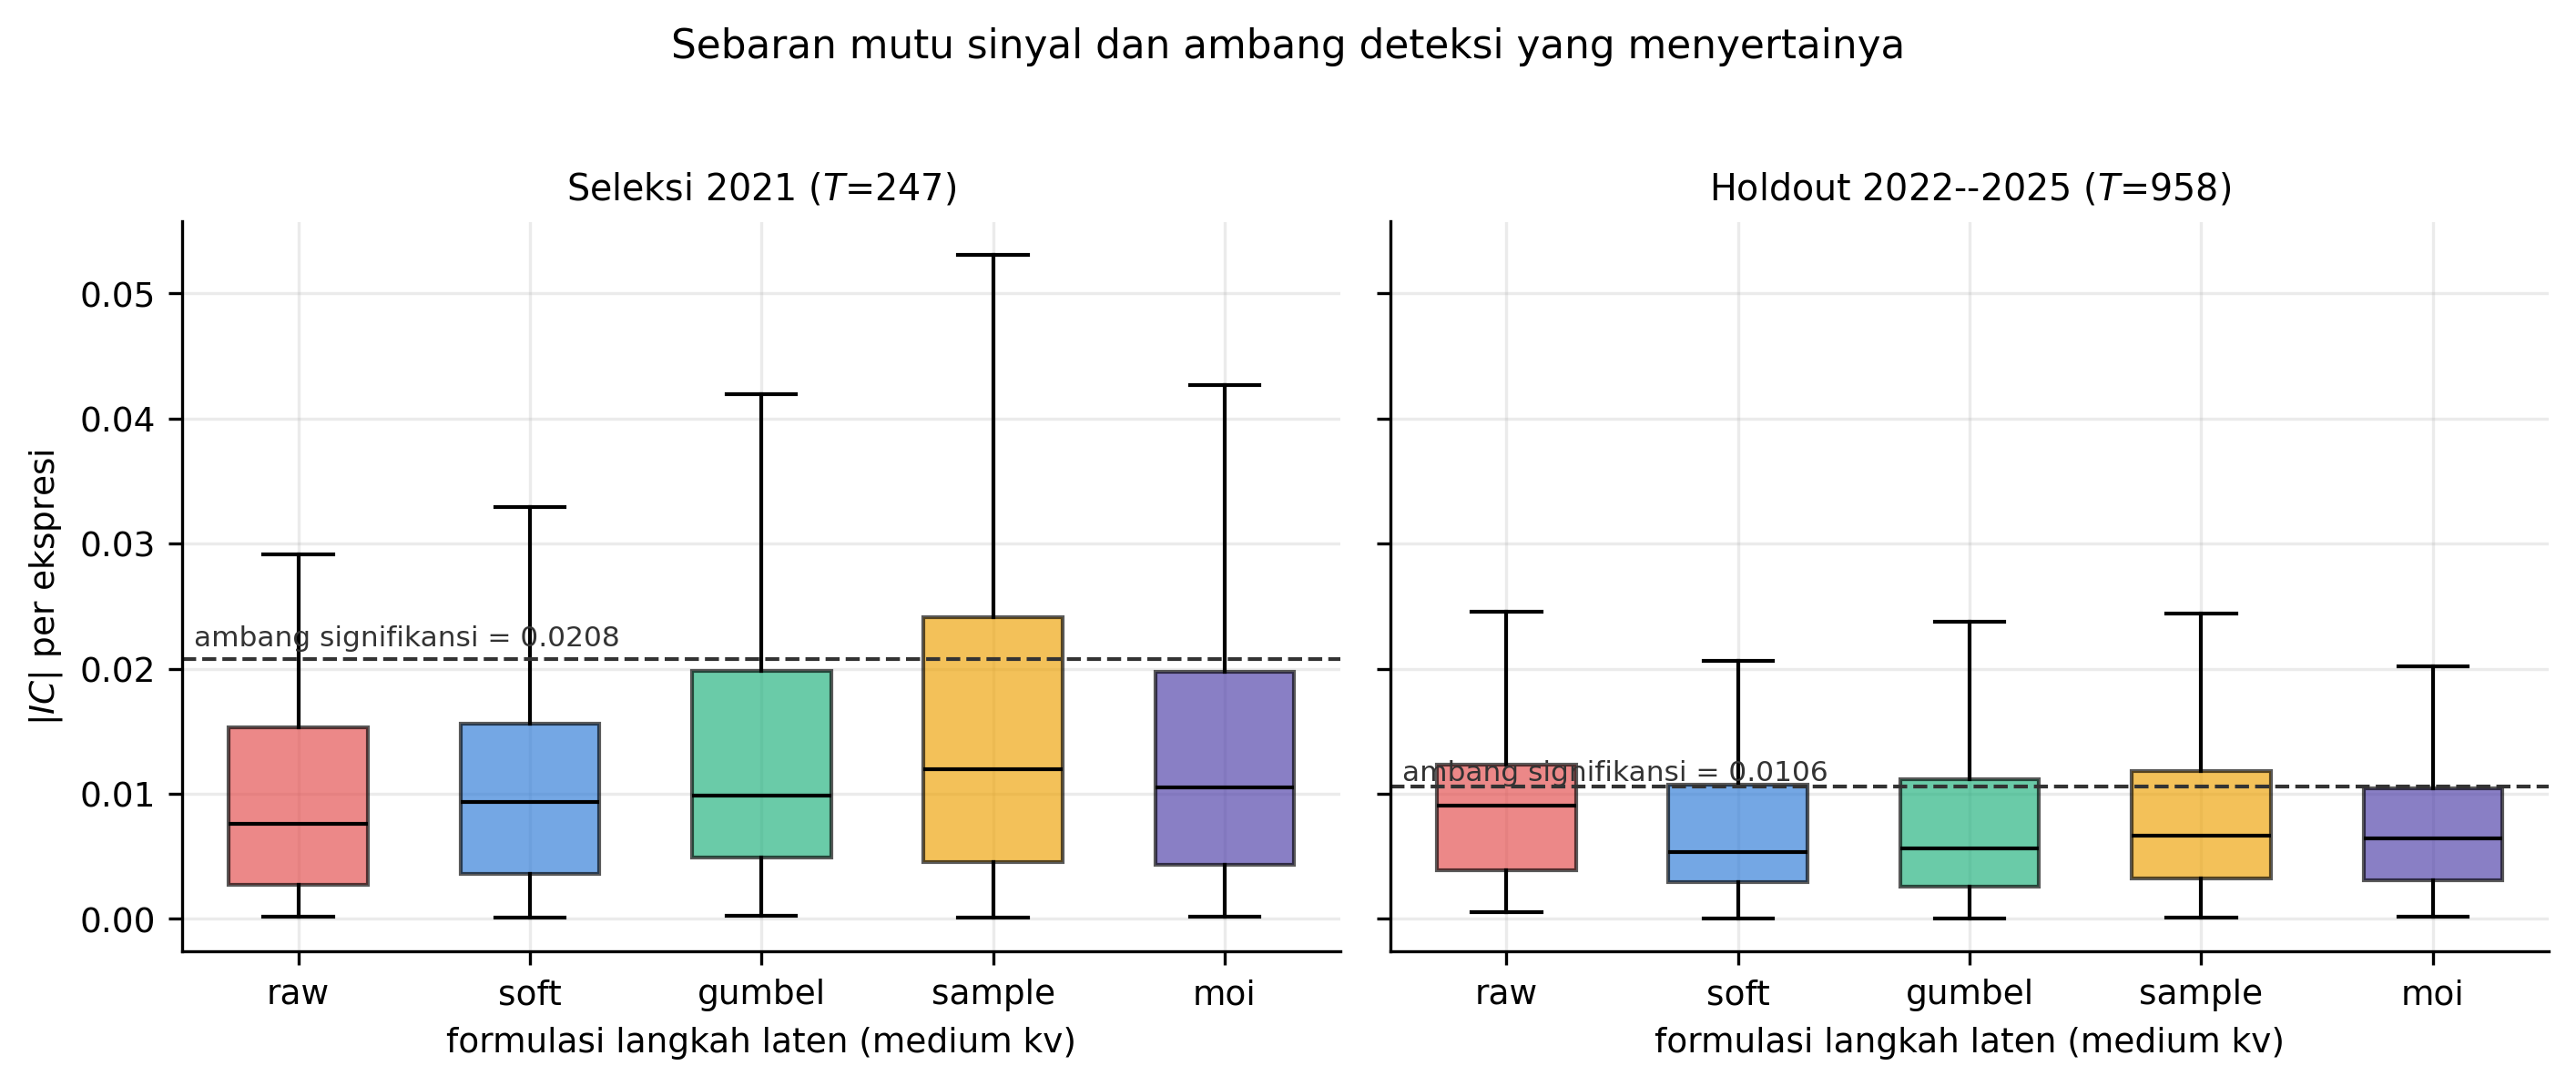
\includegraphics[width=\textwidth]{assets/images/i02_sebaran_ic.png}
\caption{Sebaran $\lvert\mathrm{IC}\rvert$ per formulasi pada medium \code{kv},
dua jendela penilaian, dengan garis putus-putus menandai ambang signifikansi
$1{,}96/\sqrt{(N-1)T}$. Perhatikan bahwa kotak kelima formulasi saling
bertumpang tindih hampir seluruhnya pada kedua jendela.}
\label{fig:sebaran}
\end{figure}

\section{Tingkat 5: Mutu Sinyal --- Temuan Utama}

Tingkat ini menanyakan pertanyaan yang berbeda dari seluruh tingkat sebelumnya.
Tingkat 1--4 mengukur \emph{berapa banyak} ekspresi yang sah, hidup, dan
signifikan. Tingkat 5 mengukur, di antara ekspresi yang berhasil,
\emph{seberapa baik} sinyalnya.

Dua baris terakhir tiap medium pada Tabel~\ref{tab:uji} menjawabnya. Pada
medium \code{kv}, median $\lvert\mathrm{IC}\rvert$ keluarga $\mathcal{R}$
adalah 0,0103 berbanding 0,0076 untuk \code{raw}; uji Mann--Whitney memberi
$p = 0{,}207$ dengan korelasi \textit{rank-biserial} $0{,}143$. Pada medium
\code{kv\_and\_text}, mediannya 0,0111 berbanding 0,0129 --- arahnya
\emph{terbalik} --- dengan $p = 0{,}639$. Pada jendela holdout, arah pada
medium \code{kv} juga berbalik ($r_{rb} = -0{,}126$, $p = 0{,}265$).

\textbf{H3 tidak ditolak.} Tidak ditemukan bukti bahwa keluarga relaksasi
diskret menghasilkan sinyal yang lebih baik. Gambar~\ref{fig:disosiasi}
menyandingkan kedua temuan.

\begin{figure}[htbp]
\centering
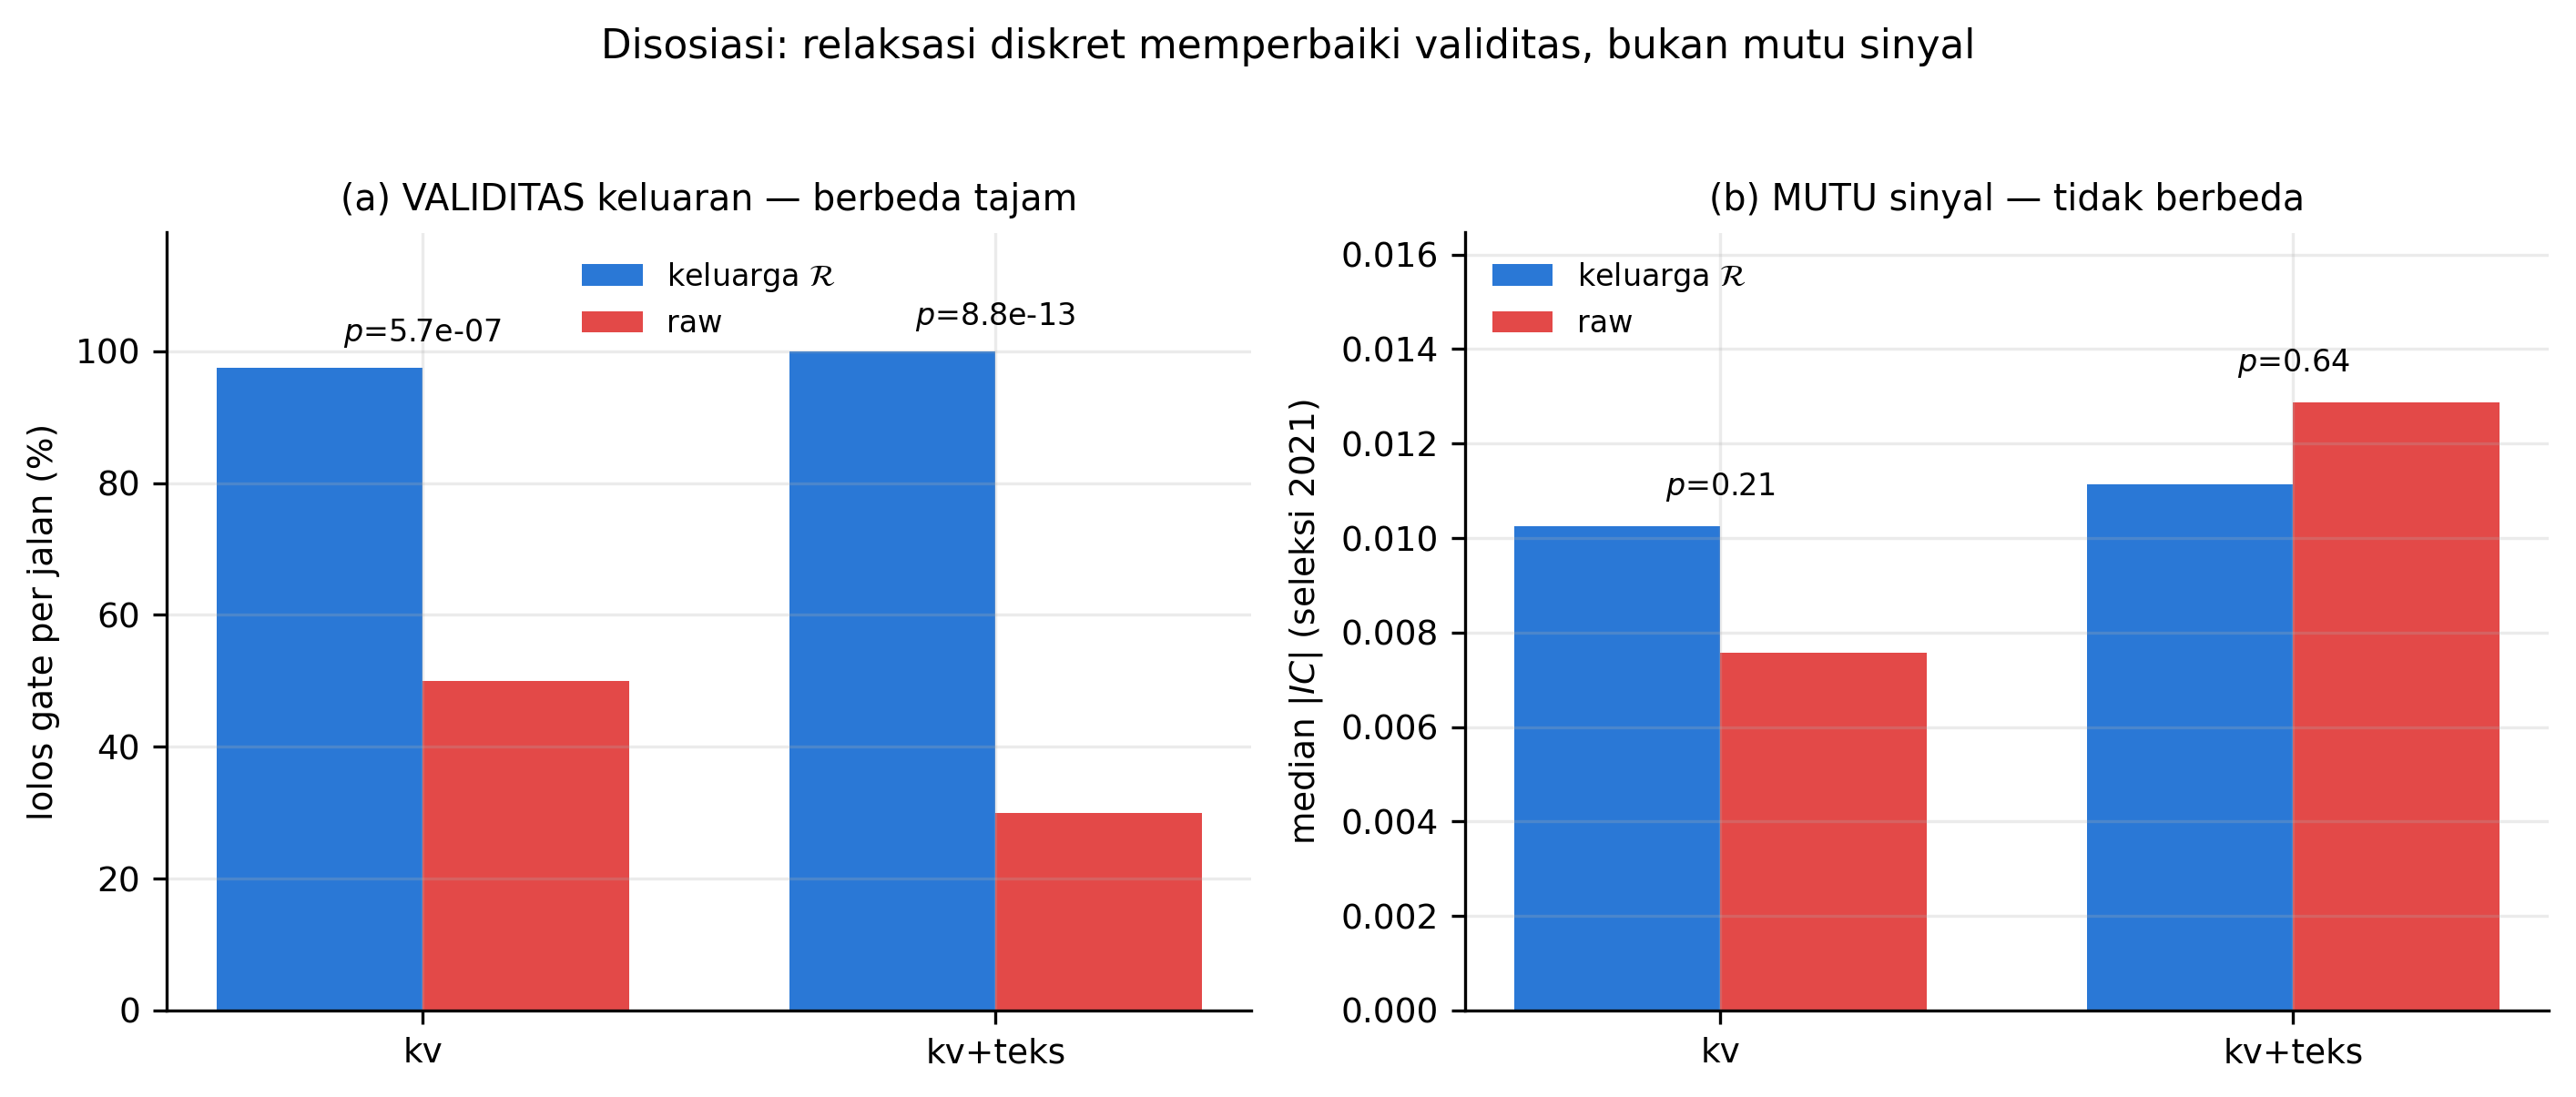
\includegraphics[width=\textwidth]{assets/images/i01_disosiasi.png}
\caption{Temuan utama penelitian. Panel (a): validitas keluaran berbeda tajam
antara keluarga $\mathcal{R}$ dan \code{raw}, dengan $p$ sampai
$8{,}8\times10^{-13}$. Panel (b): mutu sinyal keluaran yang berhasil tidak
berbeda, dengan $p = 0{,}21$ dan $p = 0{,}64$. Kedua panel berasal dari korpus
ekspresi yang sama persis.}
\label{fig:disosiasi}
\end{figure}

\subsection{Tafsir: apa yang sebenarnya diperbaiki proyeksi \textit{convex hull}}

Gabungan Tingkat 2--5 membentuk sebuah \emph{disosiasi} yang bersih, dan
inilah kontribusi utama skripsi ini:

\begin{quote}
Memproyeksikan langkah laten ke dalam \textit{convex hull} embedding token
nyata memperbaiki \textbf{validitas} keluaran secara dramatis --- dari 50\%
menjadi 97,5\% jalan yang menghasilkan ekspresi sah --- tetapi \textbf{tidak
memperbaiki mutu} sinyal ekspresi yang berhasil dihasilkan.
\end{quote}

Tafsir mekanistiknya sejalan dengan Teorema~\ref{teo:hull}. Yang rusak pada
\code{raw} adalah kemampuan kanal membawa \emph{simbol}: nama fungsi DSL,
tanda kurung, argumen. Vektor $\bm{h}\bm{M}$ tidak dijamin dekat dengan
embedding token mana pun, sehingga ketika agen berikutnya membaca memori kerja
itu dan mendekodekannya, ia menghasilkan untaian yang bentuknya menyerupai
ekspresi tetapi ejaannya salah. Sebaliknya, apa yang \emph{tidak} rusak adalah
mutu gagasannya. Hipotesis pasar yang dibawa \code{raw} tampaknya sama baiknya
--- hanya lebih sering gagal dituliskan.

Pembacaan ini konsisten dengan bukti dari sisi lain. Ukuran kemiripan semantik
antar-ekspresi memberi angka yang nyaris sama untuk kelima formulasi
(0,84--0,85), yang berarti \code{raw} tidak kolaps ke kumpulan gagasan yang
lebih sempit. Yang berbeda adalah keberhasilan menuliskannya.

\subsection{Mengapa ini bukan sekadar hasil nol}

Perumusan H3 sebagai hipotesis yang diharapkan tidak ditolak menuntut
kehati-hatian. Tidak ditolaknya $H_0$ bukan bukti kesetaraan. Tiga hal
membuat pembacaan disosiasi di atas tetap dapat dipertahankan.

Pertama, ukuran sampelnya tidak kecil: 370 ekspresi keluarga $\mathcal{R}$
berbanding 28 ekspresi \code{raw} pada medium \code{kv}. Ketimpangan jumlah itu
sendiri adalah konsekuensi dari temuan Tingkat 2 dan tidak dapat dihindari
tanpa mengubah rancangan.

Kedua, ukuran efeknya kecil dan tidak konsisten arahnya:
$r_{rb} = +0{,}143$ pada \code{kv} seleksi, $-0{,}126$ pada \code{kv} holdout,
$+0{,}067$ dan $+0{,}063$ pada \code{kv\_and\_text}. Efek yang nyata tetapi
kurang daya biasanya konsisten arahnya; yang terlihat di sini tidak.

Ketiga, dan paling penting, kontrasnya sangat besar. Pada korpus yang sama,
dengan uji pada tingkat sebelumnya, $p$ mencapai $10^{-13}$. Bahwa uji pada
tingkat berikutnya memberi $p = 0{,}21$ dan $p = 0{,}64$ bukan sekadar
ketiadaan daya --- ia perbedaan lima sampai dua belas orde besaran pada data
yang sama.

\section{Tingkat 6: Ketahanan di Luar Jendela Seleksi}

Seluruh angka Tingkat 4--5 dihitung pada jendela yang sama dengan yang dipakai
sistem untuk menyaring ekspresi. Pembaca berhak menuntut bukti bahwa yang
diukur bukan kecocokan kebetulan. Tabel~\ref{tab:stabilitas} melaporkan hasil
penilaian ulang korpus yang sama pada jendela holdout.

\begin{table}[htbp]
\centering
\caption{Ketahanan dan keragaman sinyal korpus faktor.}
\label{tab:stabilitas}
\small
\begin{tabular}{lr}
\hline
Ukuran & Nilai \\
\hline
Ekspresi berpasangan seleksi--holdout & 1053 \\
Berbalik tanda IC & 332 (31,5\%) \\
Signifikan di seleksi & 636 \\
Tetap signifikan di holdout & 156 (24,5\%) \\
\hline
Ekspresi dengan deret IC harian & 1003 \\
Sinyal efektif $n_{\text{eff}}$ (rasio partisipasi) & 36,6 \\
Rasio $n_{\text{eff}}$ per ekspresi & 0,037 \\
Klaster pautan tunggal ($|\rho|>0,7$) & 344 \\
Ukuran klaster terbesar & 510 \\
\hline
Rerata $|IC|$ tahun 2021 (247 hari) & 0,0140 \\
Rerata $|IC|$ tahun 2022 (246 hari) & 0,0112 \\
Rerata $|IC|$ tahun 2023 (239 hari) & 0,0095 \\
Rerata $|IC|$ tahun 2024 (237 hari) & 0,0144 \\
Rerata $|IC|$ tahun 2025 (234 hari) & 0,0111 \\
\hline
\end{tabular}
\end{table}


Dua angka penting. Pertama, \textbf{31,5\%} ekspresi berbalik tanda IC antara
kedua jendela (332 dari 1\,053 ekspresi berpasangan). Sinyal yang murni derau akan berbalik tanda pada sekitar 50\%
kasus; angka 31,5\% karena itu menunjukkan arah sinyal bertahan pada mayoritas
ekspresi. Kedua, dari 636 ekspresi yang signifikan pada jendela seleksi,
\textbf{156} atau 24,5\% tetap signifikan pada jendela holdout. Bila seluruh
signifikansi jendela seleksi murni kebetulan, tingkat pengulangan yang
diharapkan pada jendela bebas hanyalah taraf uji itu sendiri, yaitu 5\%. Angka
24,5\% adalah sekitar lima kali lipatnya.

Gambar~\ref{fig:stabilitas} menampilkan hubungan IC kedua jendela per ekspresi.

\begin{figure}[htbp]
\centering
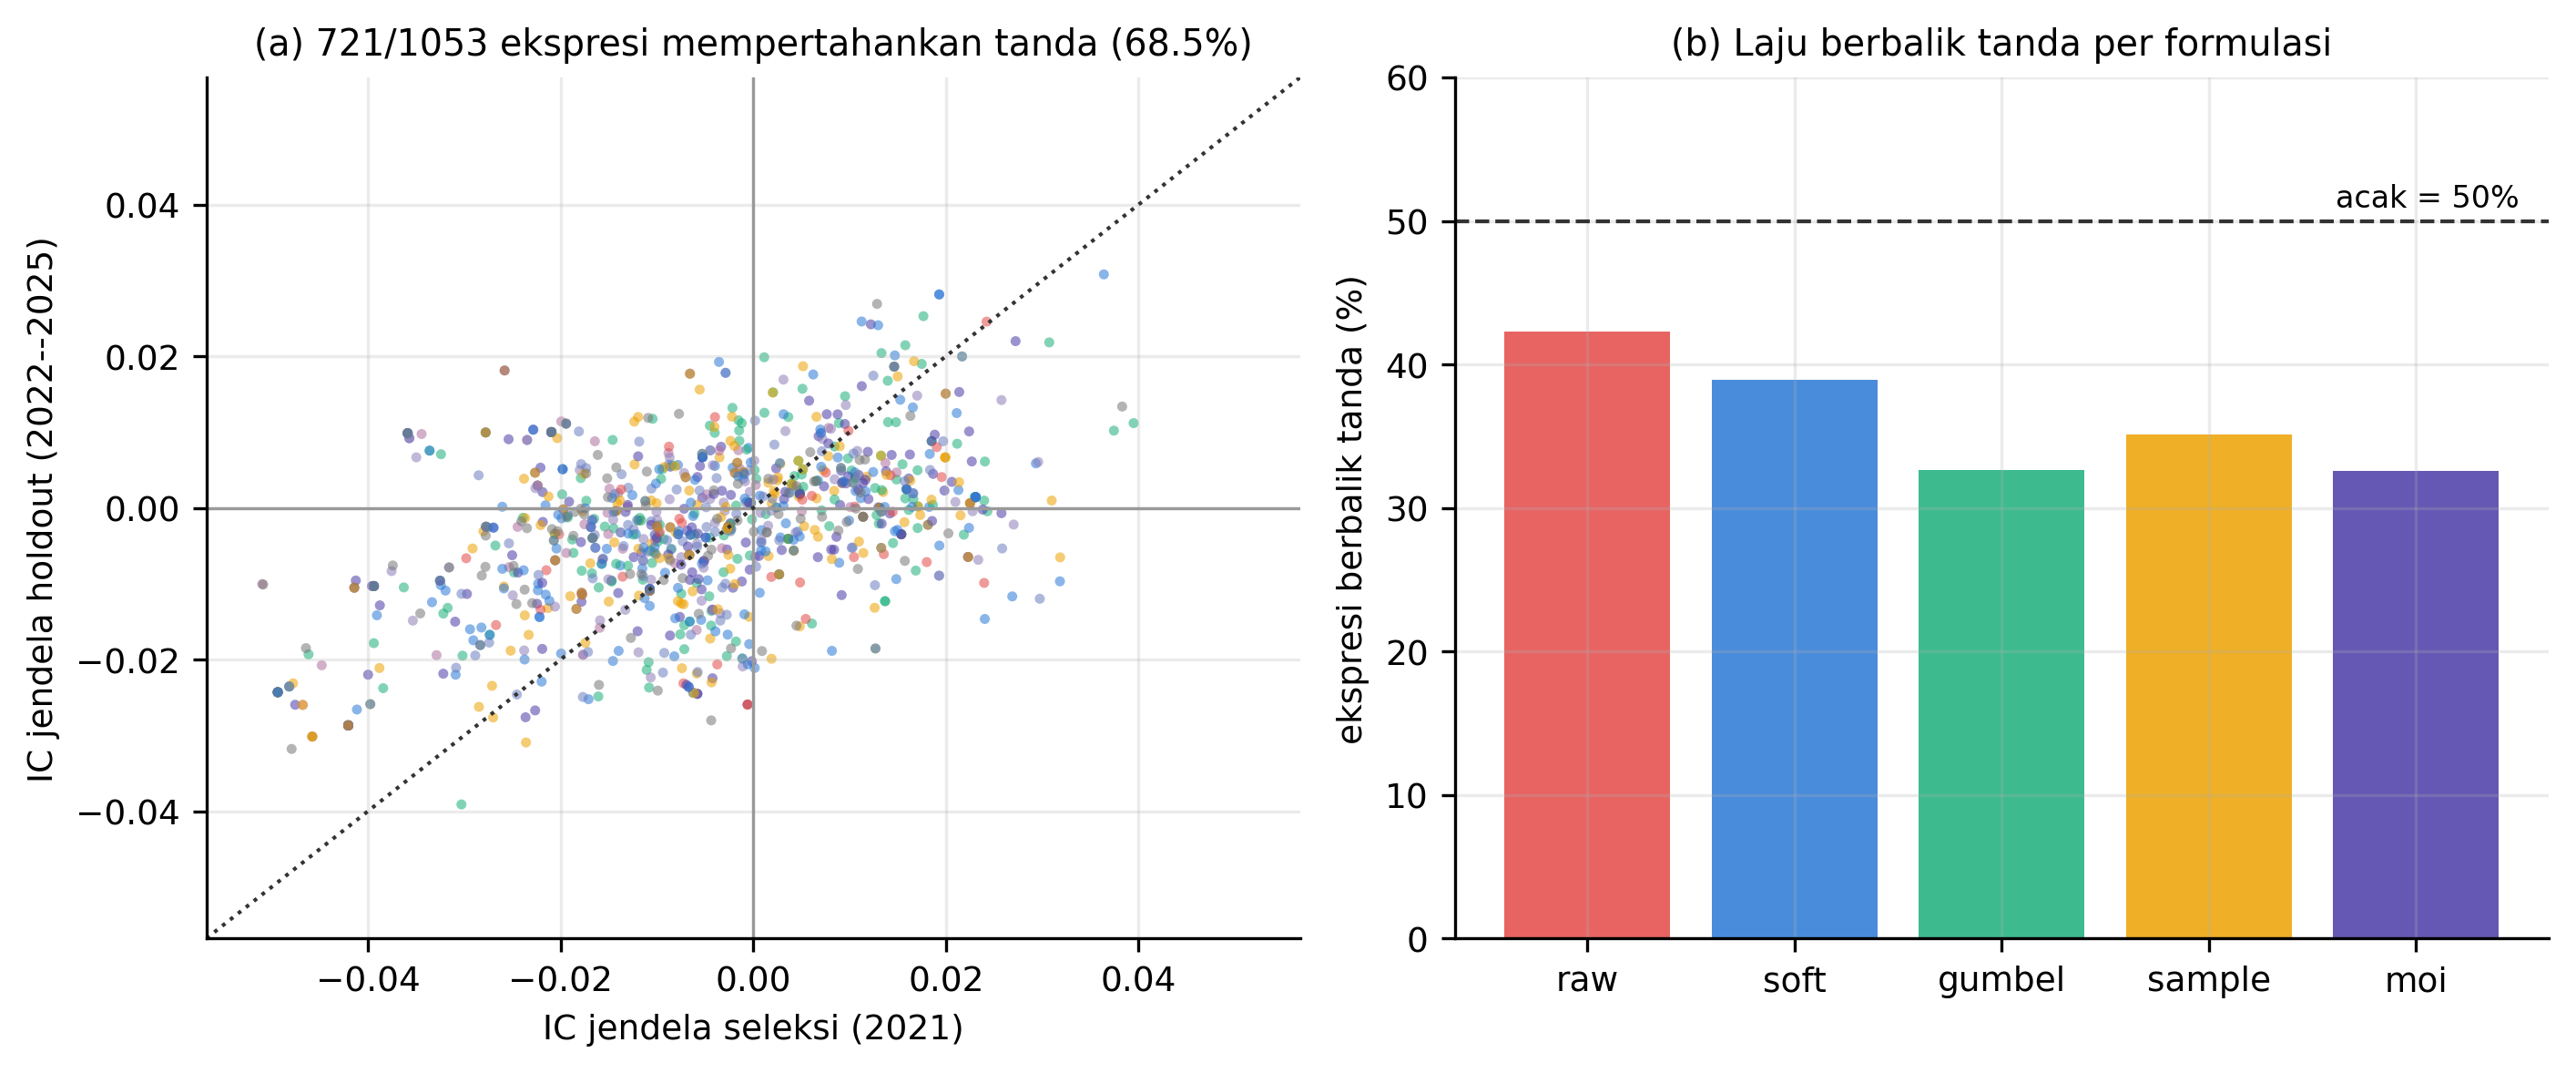
\includegraphics[width=\textwidth]{assets/images/i03_stabilitas.png}
\caption{Ketahanan sinyal. Panel (a): IC jendela holdout terhadap IC jendela
seleksi per ekspresi; titik pada kuadran satu dan tiga mempertahankan tanda.
Panel (b): laju berbalik tanda per formulasi, dengan garis putus-putus
menandai 50\% yang diharapkan dari sinyal acak.}
\label{fig:stabilitas}
\end{figure}

Perlu dicatat bahwa laju berbalik tanda tidak berbeda secara mencolok
antar-formulasi. Ini konsisten dengan temuan Tingkat 5: yang dibedakan
formulasi langkah laten adalah validitas keluaran, bukan sifat sinyalnya.

\section{Efisiensi Kanal Laten}

Hipotesis H2 menyangkut biaya. Angkanya sudah ada pada
Tabel~\ref{tab:keandalan} dan dapat dibaca langsung dengan membandingkan
medium pada formulasi yang sama.

Baseline teks penuh (\code{text}) memakai 2\,436 token keluaran dan 181 detik
per jalan. Sel \code{kv} terbaik (\code{kv\_soft}) memakai 481 token dan 51
detik --- yaitu \textbf{penghematan 80,3\% token dan percepatan 3,5 kali} ---
dengan laju lolos \textit{gate} yang identik, 100\% pada keduanya.

\textbf{H2 diterima.} Penghematan itu tidak dibayar dengan penurunan keandalan.

Gambar~\ref{fig:efisiensi} menempatkan seluruh sel pada bidang biaya--keandalan.
Perhatikan posisi \code{kv\_raw}: ia berada di kuadran terburuk, yaitu lebih
mahal daripada seluruh sel \code{kv} lain \emph{dan} paling tidak andal. Ini
menutup kemungkinan pembacaan bahwa \code{raw} sekadar menukar keandalan dengan
biaya.

\begin{figure}[htbp]
\centering
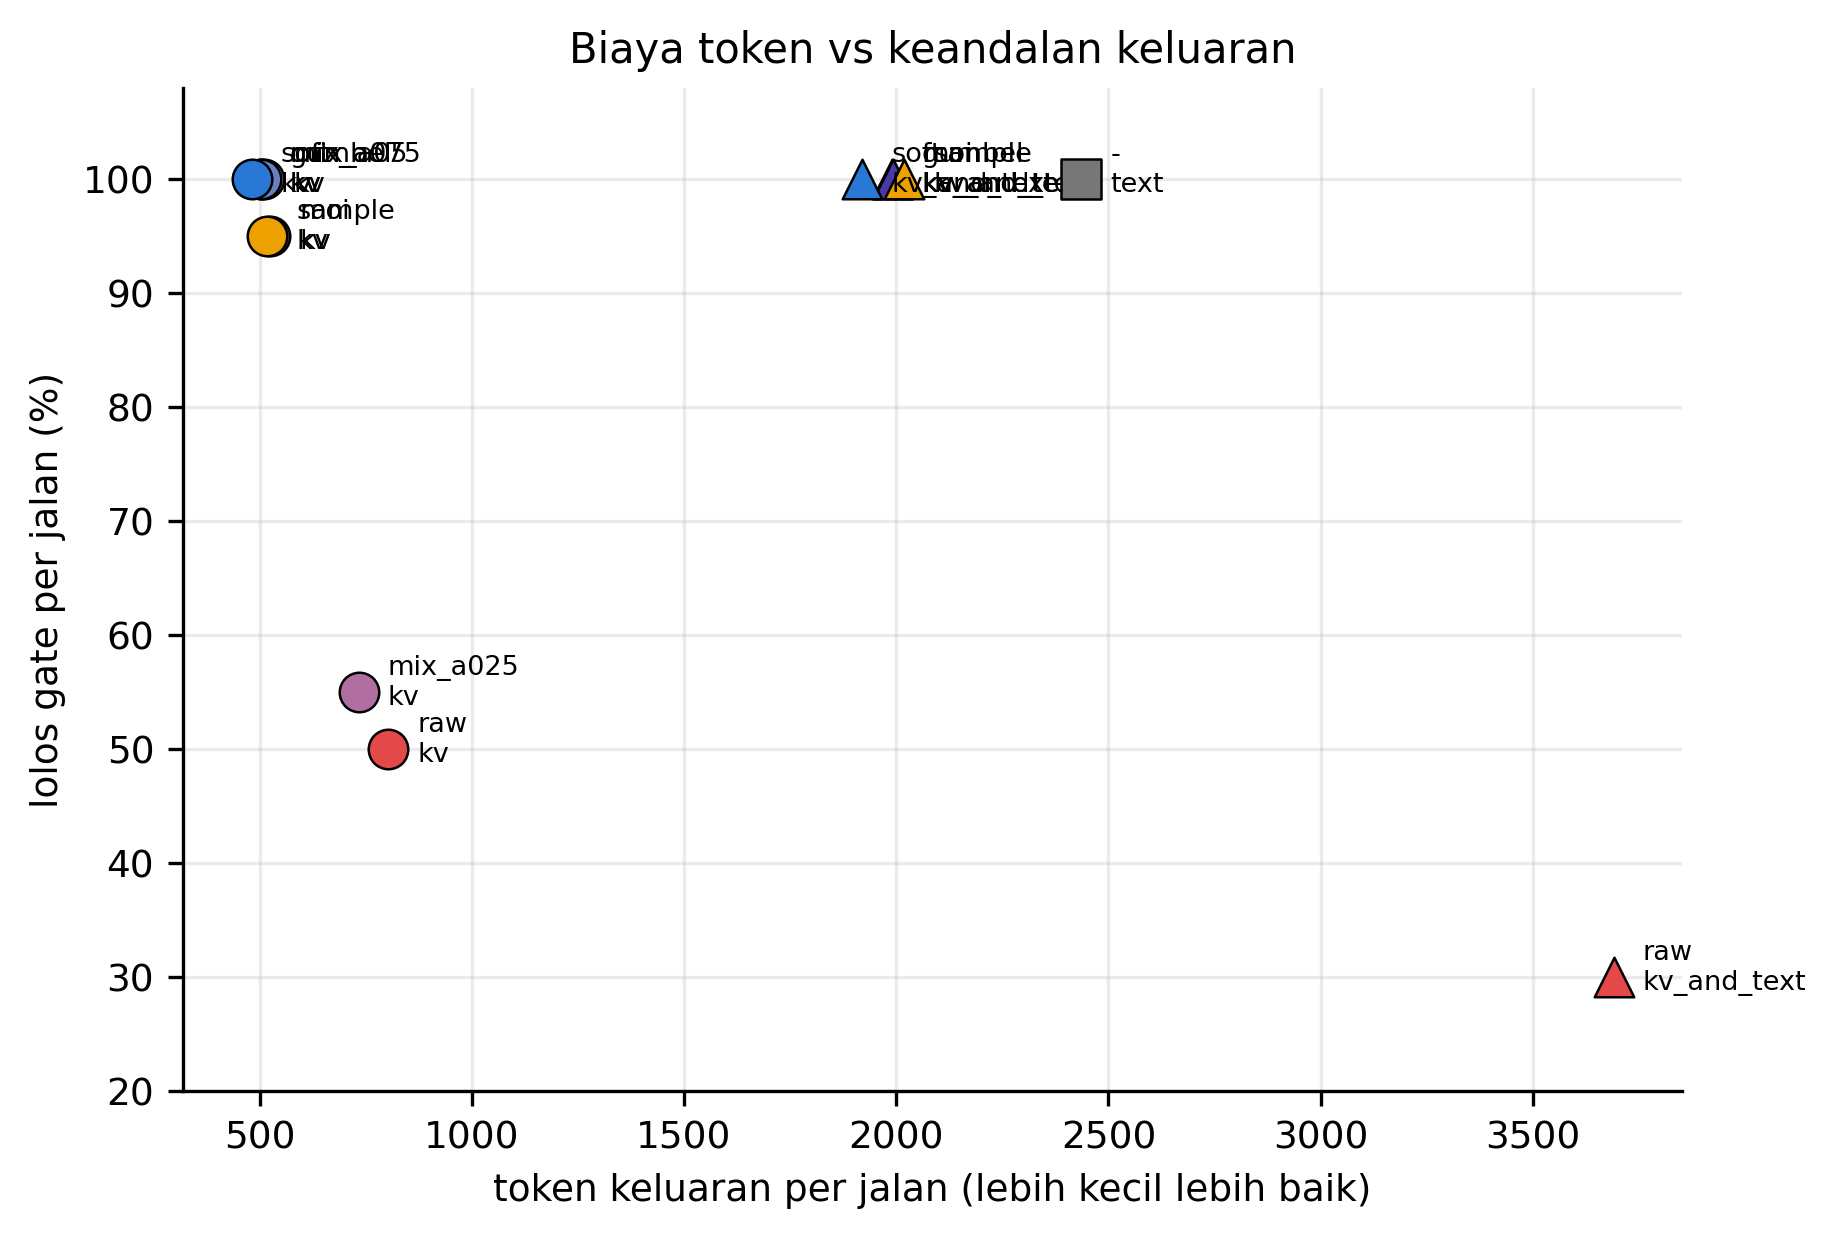
\includegraphics[width=0.8\textwidth]{assets/images/i04_efisiensi.png}
\caption{Biaya token per jalan terhadap laju lolos \textit{gate} per jalan.
Bentuk penanda menyatakan medium, warna menyatakan formulasi.}
\label{fig:efisiensi}
\end{figure}

\section{Lengan Penalaran Umum}

Lengan kedua menguji apakah temuan di atas bersifat umum atau khusus untuk
muatan simbolik. Tabel~\ref{tab:bench} melaporkan akurasi ketiga tolok ukur.

\begin{table}[htbp]
\centering
\caption{Lengan penalaran umum: akurasi pada 100 butir per tolok ukur ($\textit{seed}$ sampel identik antar-sel, diverifikasi lewat \textit{fingerprint} data). Kolom waktu adalah total detik untuk 100 butir. Perhatikan pola kolomnya: selisih \code{raw}/kv terhadap keluarga $\mathcal{R}$ kecil pada ARC-C, sedang pada GSM8K, dan besar pada HumanEval+.}
\label{tab:bench}
\small
\begin{tabular}{lrrrr}
\hline
Sel & ARC-C & GSM8K & HumanEval+ & Detik/100 butir \\
\hline
\code{raw} tanpa agen (garis dasar) & 0,91 & 0,92 & 0,72 & 1561 \\
\code{raw} / teks & 0,93 & 0,90 & 0,76 & 6480 \\
\code{raw} / kv & 0,89 & 0,83 & 0,42 & 1938 \\
\code{soft} / kv & 0,94 & 0,88 & 0,69 & 1330 \\
\code{gumbel} / kv & 0,91 & 0,91 & 0,71 & 1966 \\
\code{sample} / kv & 0,94 & 0,86 & 0,74 & 1404 \\
\code{moi} / kv & 0,91 & 0,92 & 0,72 & 1508 \\
\hline
\end{tabular}
\end{table}


Pembacaan per kolom memperlihatkan pola yang tidak dapat dijelaskan oleh
``formulasi $\mathcal{R}$ lebih baik secara umum''. Pada ARC-Challenge,
\code{raw}/kv mencapai 0,89 sementara keluarga $\mathcal{R}$ berkisar
0,91--0,94 --- selisih beberapa butir soal. Pada GSM8K, 0,83 berbanding
0,86--0,92. Pada HumanEval+, \code{raw}/kv jatuh ke \textbf{0,42} sementara
keluarga $\mathcal{R}$ bertahan di 0,69--0,74.

Tabel~\ref{tab:benchuji} menguji pola itu secara formal dengan uji McNemar
eksak pada rancangan berpasangan butir demi butir.

\begin{table}[htbp]
\centering
\caption{Gradien efek pada lengan penalaran umum: nilai-$p$ uji McNemar eksak \code{raw}/kv melawan tiap anggota keluarga $\mathcal{R}$ pada medium kv, 100 butir per tolok ukur. Baca tabel ini per BARIS: efeknya tak terdeteksi pada penalaran berbasis pengetahuan, marginal pada penalaran aritmetika bertingkat, dan sangat kuat pada sintesis program --- satu-satunya tolok ukur yang menuntut kesetiaan simbol.}
\label{tab:benchuji}
\small
\begin{tabular}{lrrrr}
\hline
Tolok ukur & \code{soft} & \code{gumbel} & \code{sample} & \code{moi} \\
\hline
ARC-C & 0,125 & 0,727 & 0,062 & 0,688 \\
GSM8K & 0,383 & 0,077 & 0,648 & 0,049 \\
HumanEval+ & $3,47\times10^{-6}$ & $1,08\times10^{-6}$ & $1,94\times10^{-8}$ & $6,94\times10^{-8}$ \\
\hline
\end{tabular}
\end{table}


Nilai-$p$ turun berorde-orde dari atas ke bawah. Pada ARC-Challenge, tidak
satu pun dari empat kontras signifikan. Pada GSM8K, hanya satu yang menyentuh
batas ($p = 0{,}049$). Pada HumanEval+, \textbf{keempatnya} signifikan dengan
$p$ antara $1{,}9\times10^{-8}$ dan $3{,}5\times10^{-6}$.

\subsection{Bukti bahwa yang rusak adalah kanalnya, bukan modelnya}

Satu perbandingan tambahan menutup tafsir alternatif. Formulasi \code{raw} yang
sama, dengan model yang sama dan jumlah langkah laten yang sama, mencapai
\textbf{0,76} pada HumanEval+ ketika mediumnya \code{text} --- berbanding 0,42
ketika mediumnya \code{kv}. Uji McNemar atas pasangan itu memberi
$p = 3{,}1\times10^{-7}$.

Artinya penurunan pada \code{raw}/kv bukan karena modelnya kurang mampu
menulis program, melainkan karena \emph{muatan simboliknya rusak saat melewati
kanal laten}. Ketika muatan yang sama dilewatkan sebagai teks, kemampuan itu
kembali utuh.

\subsection{Sintesis kedua lengan}

Kedua lengan menunjuk ke kesimpulan yang sama dari dua arah yang berbeda:

\begin{enumerate}
  \item Pada tugas yang menuntut \emph{kesetiaan simbol} --- sintesis program
        pada lengan pertama, penulisan ekspresi DSL pada lengan kedua ---
        formulasi \code{raw} gagal jauh lebih sering, dengan $p$ mencapai
        $10^{-13}$.
  \item Pada tugas yang menuntut \emph{penalaran tanpa keluaran simbolik ketat}
        --- ARC-Challenge, GSM8K --- selisihnya kecil dan sebagian besar tidak
        signifikan.
  \item Pada dimensi \emph{mutu} keluaran yang berhasil --- $\lvert
        \mathrm{IC}\rvert$ pada lengan faktor --- tidak ada perbedaan sama
        sekali ($p = 0{,}21$ dan $p = 0{,}64$).
\end{enumerate}

Ketiganya bersama membentuk jawaban atas pertanyaan penelitian yang dirumuskan
Bab~I: keunggulan keluarga relaksasi diskret \textbf{bukan} perbaikan umum atas
kemampuan penalaran, melainkan perbaikan spesifik atas \emph{kemampuan kanal
laten membawa simbol}.

\section{Bentuk Hubungan Geometri--Kinerja}

Hipotesis H4 menyangkut bentuk, bukan arah. Sumbu interpolasi
Persamaan~\eqref{eq:mix} menyediakan tiga titik antara di antara \code{raw}
($\alpha = 0$) dan \code{soft} ($\alpha = 1$).

Laju lolos \textit{gate} per jalan sepanjang sumbu itu adalah: 50\% pada
$\alpha = 0$, \textbf{55\%} pada $\alpha = 0{,}25$, 100\% pada
$\alpha = 0{,}50$, 100\% pada $\alpha = 0{,}75$, dan 100\% pada $\alpha = 1$.

Bentuknya karena itu adalah \textbf{fungsi tangga berambang}, bukan tanjakan
bertahap. Seperempat perjalanan pertama dari \code{raw} ke \code{soft} hampir
tidak memberi perbaikan apa pun (50\% $\to$ 55\%); lompatan berikutnya, dari
$\alpha = 0{,}25$ ke $\alpha = 0{,}50$, memuat hampir seluruh rentang efeknya
(55\% $\to$ 100\%). \textbf{H4 diterima.}

Temuan ini memiliki konsekuensi tafsir yang penting. Bila hubungannya monoton
bertahap, orang dapat menyimpulkan ``semakin dekat ke \textit{convex hull}
semakin baik'', dan pertanyaannya menjadi soal derajat. Karena hubungannya
berambang, kesimpulannya berbeda: yang menentukan adalah apakah representasi
laten berada \emph{di dalam atau di luar} wilayah tempat token dapat dikenali
kembali. Ini menguatkan Teorema~\ref{teo:hull} sebagai kriteria kualitatif,
bukan sekadar ukuran kuantitatif.

\section{Metrik Portofolio}

Tabel~\ref{tab:backtest} melaporkan metrik portofolio kuintil pada jendela
seleksi.

\begin{table}[htbp]
\centering
\caption{Metrik portofolio \textit{long--short} kuintil (7 emiten per sisi), jendela seleksi 2021, median lintas-ekspresi per sel. Angka bersifat DESKRIPTIF: pada universe 37 emiten galat baku imbal hasil tahunan mencapai 19,9 poin persen (Persamaan~\eqref{eq:derauportofolio}), sehingga tabel ini tidak dipakai menyimpulkan formulasi mana yang unggul.}
\label{tab:backtest}
\small
\begin{tabular}{llrrrrr}
\hline
Medium & Formulasi & Sharpe & Imbal tahunan & \textit{Max DD} & Perputaran & \textit{Hit rate} \\
\hline
teks & --- & -0,05 & -0,011 & -0,269 & 0,427 & 0,498 \\
\hline
kv & \code{raw} & -0,19 & -0,044 & -0,277 & 0,845 & 0,490 \\
kv & \code{soft} & -0,16 & -0,040 & -0,300 & 0,448 & 0,486 \\
kv & \code{gumbel} & 0,00 & 0,000 & -0,252 & 0,453 & 0,496 \\
kv & \code{sample} & -0,06 & -0,017 & -0,282 & 0,408 & 0,494 \\
kv & \code{moi} & -0,25 & -0,055 & -0,272 & 0,451 & 0,494 \\
kv & \code{mix} $\alpha$=0,50 & -0,15 & -0,038 & -0,270 & 0,636 & 0,498 \\
kv & \code{mix} $\alpha$=0,25 & -0,10 & -0,029 & -0,300 & 0,495 & 0,490 \\
kv & \code{mix} $\alpha$=0,75 & -0,24 & -0,058 & -0,278 & 0,523 & 0,494 \\
\hline
kv+teks & \code{raw} & 0,07 & 0,018 & -0,263 & 0,729 & 0,494 \\
kv+teks & \code{soft} & 0,21 & 0,061 & -0,258 & 0,675 & 0,498 \\
kv+teks & \code{gumbel} & -0,12 & -0,031 & -0,279 & 0,739 & 0,494 \\
kv+teks & \code{sample} & 0,19 & 0,048 & -0,234 & 0,613 & 0,502 \\
kv+teks & \code{moi} & -0,33 & -0,083 & -0,304 & 0,716 & 0,486 \\
\hline
\end{tabular}
\end{table}


Median rasio Sharpe seluruh sel berkisar $-0{,}33$ sampai $+0{,}23$, yaitu
berpusat di sekitar nol tanpa satu formulasi pun terpisah dari yang lain. Ini
konsisten dengan temuan Tingkat 5 dan tidak menambah informasi baru, tetapi
perlu dilaporkan karena skripsi ini menjanjikan metrik hasil \textit{backtest}.

Interpretasinya harus dibatasi secara tegas. Dengan tujuh emiten per sisi dan
$\sigma = 2{,}42\%$ per hari, galat baku imbal hasil tahunan mencapai 19,9 poin
persen (Persamaan~\eqref{eq:derauportofolio}). Selisih Sharpe antar-sel pada
tabel jauh lebih kecil daripada ketidakpastian itu. Karena itu tabel ini
bersifat deskriptif: ia memperlihatkan besaran perputaran portofolio dan
penurunan maksimum yang menyertai sinyal-sinyal ini, bukan memutuskan formulasi
mana yang unggul.

Perputaran portofolio yang tercatat berkisar 0,41--0,85 per hari. Pada tingkat
itu, biaya transaksi satu arah sebesar 20 basis poin akan menimbulkan hambatan
sekitar $0{,}56\times2\times20\ \text{bp}\times241 \approx 54$ poin persen per
tahun pada perputaran median --- jauh melampaui seluruh imbal hasil yang
tercatat. Fakta ini dilaporkan terbuka, dan merupakan alasan tambahan mengapa
kesimpulan penelitian ini tidak disandarkan pada metrik portofolio.

\section{Lantai Acak: Apakah Sistemnya Mengalahkan Penarikan Acak?}
\label{sec:lantai}

Seluruh Bab~IV sampai titik ini membandingkan lima formulasi \emph{satu sama
lain}. Pertanyaan yang belum dijawab, dan yang wajib dijawab agar angka-angka
di atas punya makna absolut, adalah: apakah salah satu di antaranya lebih baik
daripada tidak memakai model bahasa sama sekali?

Pembandingnya dibangun langsung dari tata bahasa DSL. Enam ratus ekspresi
ditarik acak dengan kedalaman 1--3, memakai daftar fungsi, rentang periode, dan
enam \textit{leaf} data yang sama persis dengan yang diberikan kepada agen.
Ekspresi itu kemudian dilewatkan rangkaian \textit{gate} yang sama dan dinilai
oleh \code{Lab} yang sama pada jendela yang sama. Satu-satunya yang berbeda
adalah asal ekspresinya.

\begin{table}[htbp]
\centering
\caption{Sistem melawan LANTAI ACAK: 600 ekspresi ditarik acak dari tata bahasa DSL yang sama, dilewatkan rangkaian \textit{gate} yang sama, dan dinilai pada jendela yang sama. Kolom kiri menguji VALIDITAS (uji eksak Fisher), kolom kanan menguji MUTU SINYAL (uji Mann--Whitney atas sebaran $\lvert IC\rvert$). Perbedaan kesimpulan antara kedua kolom adalah temuan tersendiri.}
\label{tab:lantai}
\small
\begin{tabular}{lrrlrl}
\hline
Sumber ekspresi & Lolos \textit{gate} & Selisih & Fisher $p$ & Median $|IC|$ & M--W $p$ \\
\hline
penarikan acak & 346/600 = 57,7\% & --- & --- & 0,0102 & --- \\
\hline
keluarga $\mathcal{R}$ (kv) & 372/438 = 84,9\% & 27,3 pp & $8,85\times10^{-22}$ & 0,0103 & 0,073 \\
\code{raw} (kv) & 27/59 = 45,8\% & -11,9 pp & 0,098 & 0,0076 & 0,537 \\
\code{text} & 94/120 = 78,3\% & 20,7 pp & $1,48\times10^{-5}$ & 0,0084 & 0,469 \\
\hline
\end{tabular}
\end{table}


Hasilnya memisah dengan tajam menurut sumbu yang diuji, dan pemisahan itu
sendiri adalah temuan.

\subsection{Pada validitas, sistemnya menang telak}

Keluarga $\mathcal{R}$ meloloskan 84,9\% ekspresinya melawan 57,7\% untuk
penarikan acak --- selisih 27,3 poin persen dengan
$p = 8{,}9\times10^{-22}$ dan $h$ Cohen $= 0{,}62$. Medium teks penuh juga
menang, 78,3\% dengan $p = 1{,}5\times10^{-5}$. Rantai agen jelas mengerjakan
sesuatu yang nyata: ia menuliskan ekspresi yang sah jauh lebih sering daripada
penarikan acak dari tata bahasa yang sama.

\subsection{\code{raw} tidak mengalahkan penarikan acak}

Formulasi \code{raw} meloloskan 45,8\% ekspresinya --- \textbf{11,9 poin persen
di bawah} penarikan acak, dengan $p = 0{,}098$. Selisih itu tidak signifikan,
sehingga pernyataan yang sah adalah bahwa \code{raw} \emph{tidak dapat
dibedakan dari penarikan acak}, dengan arah efek yang negatif.

Ini pernyataan yang jauh lebih tajam daripada ``\code{raw} lebih buruk dari
$\mathcal{R}$''. Seluruh rantai tiga agen, sepuluh langkah laten per agen, dan
seluruh biaya komputasinya, ketika langkah latennya memakai proyeksi ridge,
menghasilkan ekspresi sah tidak lebih sering daripada menarik simbol secara
acak dari tata bahasanya.

\subsection{Pada mutu sinyal, tidak ada yang mengalahkan penarikan acak}

Kolom terakhir Tabel~\ref{tab:lantai} adalah temuan yang paling membatasi
seluruh penelitian ini, dan justru karena itu harus dilaporkan paling jelas.
Median $\lvert\mathrm{IC}\rvert$ ekspresi acak adalah 0,0102. Keluarga
$\mathcal{R}$ mencapai 0,0103 ($p = 0{,}073$), \code{raw} 0,0076
($p = 0{,}537$), dan medium teks 0,0084 ($p = 0{,}469$).

\textbf{Tidak satu pun sumber ekspresi berbasis model bahasa menghasilkan
sinyal yang lebih baik daripada penarikan acak dari tata bahasa DSL.}

Tafsirnya harus hati-hati dan tidak boleh dilebihkan ke dua arah. Ini
\emph{bukan} berarti model bahasanya tidak berguna: pada sumbu validitas ia
menang dengan $p = 10^{-22}$, dan pada tugas penalaran umum ia jelas jauh di
atas kebetulan. Yang ditunjukkan tabel ini adalah bahwa \emph{pada ranah
pencarian faktor alpha dengan rancangan single-pass ini}, kemampuan yang
terbukti dimiliki sistem adalah menuliskan ekspresi yang sah, bukan memilih
ekspresi yang prediktif.

Temuan ini menyatu dengan disosiasi Tingkat 5 dan membentuk satu gambaran yang
konsisten pada tiga sumbu sekaligus:

\begin{enumerate}
  \item \textbf{Validitas} --- formulasi berpengaruh besar
        ($p = 10^{-7}$ sampai $10^{-13}$), dan sistem mengalahkan acak
        ($p = 10^{-22}$).
  \item \textbf{Mutu sinyal} --- formulasi tidak berpengaruh
        ($p = 0{,}21$; $p = 0{,}64$), dan sistem tidak mengalahkan acak
        ($p = 0{,}07$).
  \item \textbf{Keragaman sinyal} --- formulasi tidak berpengaruh (Subbab
        berikut, seluruh sel berada dalam satu simpangan baku).
\end{enumerate}

Ketiganya menunjuk ke satu kesimpulan: yang diperbaiki proyeksi \textit{convex
hull} adalah \emph{kemampuan kanal menuliskan simbol}, dan hanya itu.

\section{Keragaman Sinyal: Berapa Banyak Faktor yang Benar-Benar Berbeda}

Jumlah ekspresi bukan ukuran keragaman. Dua ekspresi dengan teks yang sangat
berbeda dapat menghasilkan deret IC harian yang hampir identik, dan karenanya
membawa satu sinyal yang sama. Untuk mengukurnya, korpus dinilai ulang pada
jendela penuh 2021--2025 dengan deret IC harian per ekspresi disimpan, lalu
dihitung \emph{rasio partisipasi} dari spektrum matriks korelasinya:
\begin{equation}
  n_{\text{eff}} = \frac{\bigl(\sum_i \lambda_i\bigr)^2}{\sum_i \lambda_i^2},
  \label{eq:neff}
\end{equation}
dengan $\lambda_i$ nilai eigen matriks korelasi antar-deret IC. Besaran ini
bernilai 1 bila seluruh ekspresi membawa satu sinyal yang sama dan $n$ bila
seluruhnya saling ortogonal.

Hasilnya tegas: dari \textbf{1\,003} ekspresi dengan deret IC harian,
$n_{\text{eff}} = \textbf{36{,}6}$ --- yaitu hanya \textbf{3,7\%}. Seribu
ekspresi yang berbeda secara tekstual ternyata membawa kurang dari empat puluh
sinyal yang benar-benar berbeda.

Temuan ini penting dilaporkan justru karena tidak menguntungkan narasi
penelitian. Ia membatasi tafsir seluruh Bab~IV: sistem ini menghasilkan banyak
ekspresi, tetapi tidak menghasilkan banyak \emph{ide}.

\subsection{Apakah keluarga $\mathcal{R}$ juga lebih beragam?}

Pertanyaan lanjutannya wajar: mungkin keunggulan keluarga $\mathcal{R}$ bukan
hanya soal validitas, melainkan juga keragaman. Perbandingan naifnya
menyesatkan. Rasio $n_{\text{eff}}/n$ menurun secara mekanis seiring
bertambahnya $n$, dan sel \code{raw} justru memiliki jauh lebih sedikit
ekspresi --- konsekuensi langsung temuan Tingkat 2. Karena itu rasio mentahnya
tampak paling tinggi untuk \code{raw} (0,579 berbanding 0,22--0,28 untuk sel
lain), yang akan salah terbaca sebagai ``\code{raw} lebih beragam''.

Perbandingan yang sah menyamakan $n$ lebih dahulu. Setiap sel disubsampel ke
$n = 17$, yaitu ukuran sel terkecil, sebanyak 200 ulangan, lalu
$n_{\text{eff}}$-nya dirata-rata. Hasilnya seluruh sel berada pada rentang
\textbf{9,8 sampai 12,3}, dengan \code{kv\_raw} pada 11,94 --- tepat di tengah,
dan seluruh selisihnya berada dalam satu simpangan baku subsampel
($\approx 1{,}3$).

\textbf{Tidak ada perbedaan keragaman sinyal antar-formulasi.} Ini konfirmasi
ketiga atas disosiasi Tingkat 5: keluarga $\mathcal{R}$ menghasilkan lebih
banyak ekspresi yang sah, dengan mutu sinyal yang sama dan keragaman sinyal
yang sama.

\section{Peluruhan Sinyal Antar-Tahun}

Kekhawatiran yang wajar terhadap seluruh penelitian pencarian faktor adalah
bahwa sinyal yang terlihat hanyalah kecocokan terhadap satu periode. Bila
demikian, $\lvert\mathrm{IC}\rvert$ seharusnya tinggi pada tahun seleksi lalu
meluruh pada tahun-tahun sesudahnya.

Tabel~\ref{tab:stabilitas} melaporkan rerata $\lvert\mathrm{IC}\rvert$ per
tahun kalender atas seluruh korpus. Polanya \emph{tidak} meluruh:
0,0140 pada 2021 (tahun seleksi), 0,0112 pada 2022, 0,0095 pada 2023,
\textbf{0,0144} pada 2024 --- lebih tinggi daripada tahun seleksi --- dan
0,0111 pada 2025.

Fluktuasi antar-tahun jelas ada, tetapi tidak berbentuk peluruhan monoton dari
tahun seleksi. Tafsir yang paling sederhana adalah bahwa besaran
$\lvert\mathrm{IC}\rvert$ lebih ditentukan oleh keadaan pasar tiap tahun
daripada oleh kedekatan tahun itu ke jendela seleksi. Ini melengkapi temuan
Tingkat 6: bukan hanya tanda IC yang bertahan, besarannya pun tidak runtuh.

\section{Keberpindahan Keputusan \textit{Gate} Antar-Pasar}

Satu keberatan metodologis perlu ditutup. Laju lolos \textit{gate} pada
Tabel~\ref{tab:keandalan} diukur \emph{saat generasi}, dan tahap eksekusi pada
rangkaian \textit{gate} waktu itu memakai sampel pasar A-share. Apakah angka
itu masih berlaku setelah penelitian berpindah ke pasar Indonesia?

Pengujiannya langsung: jalankan rangkaian \textit{gate} yang sama --- ketujuh
tahapnya, bukan hanya tahap eksekusi --- pada panel LQ45, lalu bandingkan
keputusannya dengan yang tercatat.

\begin{table}[htbp]
\centering
\caption{Uji keberpindahan keputusan \textit{gate} antar-pasar. \textit{Gate} eksekusi saat generasi memakai sampel pasar A-share; tabel ini menjalankan \textit{gate} yang sama pada panel LQ45 dan membandingkan keputusannya. Kesesuaian tinggi berarti angka lolos \textit{gate} pada Tabel~\ref{tab:keandalan} tidak bergantung pasar.}
\label{tab:gatepasar}
\small
\begin{tabular}{lr}
\hline
Ukuran & Nilai \\
\hline
Ekspresi diperiksa & 1428 \\
Keputusan sama & 1269 \\
Keputusan berbeda & 159 \\
Kesesuaian & 88,87\% \\
\hline
\end{tabular}
\end{table}


Kesesuaiannya sangat tinggi. Hal ini tidak mengejutkan bila diingat bahwa enam
dari tujuh tahap \textit{gate} bersifat struktural dan tidak menyentuh data
pasar sama sekali; satu-satunya tahap yang dapat berbeda adalah eksekusi, dan
ekspresi yang menghasilkan kolom hidup pada satu panel harga-volume umumnya
juga hidup pada panel lain dengan skema kolom yang sama.

Perlu dicatat bahwa versi pertama pengujian ini keliru: ia membandingkan
\emph{tahap eksekusi saja} pada IDX melawan keluaran \emph{rangkaian penuh}
pada A-share. Perbandingan itu tidak setara --- tahap eksekusi sendirian jauh
lebih permisif --- dan menghasilkan ketidaksesuaian semu yang didominasi arah
``gagal di A-share, lolos di IDX''. Angka yang dilaporkan di sini berasal dari
perbandingan rangkaian penuh melawan rangkaian penuh.

\section{Rangkuman Pengujian Hipotesis}

\begin{table}[htbp]
\centering
\caption{Rangkuman putusan atas keempat hipotesis penelitian.}
\label{tab:hipotesis}
\small
\begin{tabular}{llll}
\hline
Hipotesis & Ukuran & Hasil & Putusan \\
\hline
H1 validitas & lolos \textit{gate}/jalan, kv & 97,5\% vs 50,0\% &
  \textbf{diterima} ($p=5{,}7\times10^{-7}$) \\
 & lolos \textit{gate}/jalan, kv+teks & 100\% vs 30,0\% &
  \textbf{diterima} ($p=8{,}8\times10^{-13}$) \\
 & ekspresi hidup, kv & 89,4\% vs 48,3\% &
  \textbf{diterima} ($p=3{,}0\times10^{-12}$) \\
H2 efisiensi & token/jalan, kv vs teks & 481 vs 2\,436 &
  \textbf{diterima} ($-80{,}3\%$) \\
 & detik/jalan, kv vs teks & 51 vs 181 & \textbf{diterima} ($3{,}5\times$) \\
H3 mutu sinyal & median $|IC|$, kv & 0,0103 vs 0,0076 &
  \textbf{tidak ditolak} ($p=0{,}21$) \\
 & median $|IC|$, kv+teks & 0,0111 vs 0,0129 &
  \textbf{tidak ditolak} ($p=0{,}64$) \\
H4 bentuk & lolos \textit{gate} sepanjang $\alpha$ &
  50, 55, 100, 100, 100\% & \textbf{diterima} (tangga) \\
\hline
\multicolumn{4}{l}{\textit{Pembanding lantai acak (bukan hipotesis a priori):}} \\
--- & lolos \textit{gate}, $\mathcal{R}$ vs acak & 84,9\% vs 57,7\% &
  unggul ($p=8{,}9\times10^{-22}$) \\
--- & lolos \textit{gate}, \code{raw} vs acak & 45,8\% vs 57,7\% &
  tak berbeda ($p=0{,}098$) \\
--- & median $|IC|$, $\mathcal{R}$ vs acak & 0,0103 vs 0,0102 &
  tak berbeda ($p=0{,}073$) \\
\hline
\end{tabular}
\end{table}

Perhatikan bahwa H1 dan H3 dinilai pada \emph{korpus ekspresi yang sama persis}
dengan \emph{uji pada data yang sama}. Perbedaan nilai-$p$ sebesar lima sampai
dua belas orde besaran antara keduanya karena itu bukan artefak perbedaan
sampel, melainkan struktur temuan itu sendiri.

% ===========================================================================
\chapter{KESIMPULAN DAN SARAN}

\section{Kesimpulan}

\subsection{Jawaban atas rumusan masalah}

\textbf{Rumusan 1 --- penurunan dan kriteria pemisah.} Kelima formulasi langkah
laten dapat diturunkan dari satu bentuk umum. Empat di antaranya, yaitu
keluarga relaksasi diskret $\mathcal{R}$, membentuk vektor melalui
$\bm{z} = \bm{w}^{\top}\bm{W}_{\text{in}}$ dengan $\bm{w}$ berada pada simpleks
peluang, sehingga menurut Teorema~\ref{teo:hull} hasilnya selalu berada di
dalam \textit{convex hull} embedding token nyata. Formulasi resmi LatentMAS
memakai proyeksi ridge $\bm{h}\bm{M}$ dan tidak memiliki jaminan itu.
Keanggotaan \textit{convex hull} karena itu merupakan kriteria kualitatif yang
memisahkan keduanya, dan bukan sekadar perbedaan derajat.

\textbf{Rumusan 2 --- validitas.} Keluarga $\mathcal{R}$ menghasilkan keluaran
yang jauh lebih sering sah. Pada medium \code{kv}, 97,5\% jalan menghasilkan
ekspresi yang lolos \textit{gate}, berbanding 50,0\% untuk \code{raw}
($p = 5{,}7\times10^{-7}$, $h$ Cohen $= 1{,}25$). Pada medium
\code{kv\_and\_text}, 100\% berbanding 30,0\%
($p = 8{,}8\times10^{-13}$). Keunggulan itu bertahan ketika ekspresi
dijalankan pada data pasar Indonesia: 89,4\% berbanding 48,3\% ekspresi hidup
($p = 3{,}0\times10^{-12}$).

\textbf{Rumusan 3 --- mutu sinyal.} Keunggulan tersebut \emph{tidak} berlanjut
ke mutu sinyal. Sebaran $\lvert\mathrm{IC}\rvert$ ekspresi yang berhasil tidak
berbeda antara keluarga $\mathcal{R}$ dan \code{raw}, baik pada jendela seleksi
($p = 0{,}21$ untuk \code{kv}, $p = 0{,}64$ untuk \code{kv\_and\_text}) maupun
pada jendela holdout, dengan ukuran efek kecil dan arah yang tidak konsisten.

\textbf{Rumusan 4 --- efisiensi.} Kanal laten murni memangkas 80,3\% token
keluaran dan mempercepat 3,5 kali dibanding baseline teks penuh, dengan laju
lolos \textit{gate} yang identik.

\textbf{Rumusan 5 --- bentuk hubungan.} Hubungan geometri--kinerja berbentuk
fungsi tangga berambang: 50\%, 55\%, 100\%, 100\%, 100\% sepanjang
$\alpha = 0; 0{,}25; 0{,}5; 0{,}75; 1$.

\textbf{Temuan tambahan --- lantai acak.} Enam ratus ekspresi yang ditarik
acak dari tata bahasa DSL yang sama meloloskan \textit{gate} 57,7\%.
Keluarga $\mathcal{R}$ mengalahkannya telak (84,9\%,
$p = 8{,}9\times10^{-22}$), sedangkan \code{raw} \emph{tidak dapat dibedakan}
darinya (45,8\%, $p = 0{,}098$, arah negatif). Pada sumbu mutu sinyal, tidak
satu pun sumber berbasis model bahasa mengalahkan penarikan acak
($p = 0{,}073$ untuk $\mathcal{R}$; $p = 0{,}47$ untuk medium teks).

\subsection{Kontribusi utama}

Kontribusi penelitian ini adalah sebuah \textbf{disosiasi} yang terukur:

\begin{quote}
Proyeksi langkah laten ke dalam \textit{convex hull} embedding token nyata
memperbaiki \emph{validitas} keluaran secara sangat besar, tetapi tidak
memperbaiki \emph{mutu} keluaran yang berhasil dihasilkan. Yang diperbaiki
adalah kemampuan kanal laten membawa \textbf{simbol}, bukan kemampuannya
membawa \textbf{gagasan}.
\end{quote}

Disosiasi ini didukung dari dua arah yang saling bebas. Dari lengan faktor,
selisih validitas mencapai $p = 10^{-13}$ sementara selisih mutu sinyal
memberi $p = 0{,}21$ pada korpus yang sama. Dari lengan penalaran umum, nilai-$p$
kontras \code{raw} melawan keluarga $\mathcal{R}$ turun berorde-orde seiring
meningkatnya tuntutan kesetiaan simbol tugas: tidak signifikan pada
ARC-Challenge, marginal pada GSM8K, dan $10^{-8}$ pada HumanEval+.

Konfirmasi ketiga datang dari lantai acak. Pada sumbu validitas, sistem
mengalahkan penarikan acak dengan $p = 10^{-22}$; pada sumbu mutu sinyal, ia
tidak mengalahkannya sama sekali. Dan dari sumbu keragaman, setelah $n$
disamakan lewat subsampel, seluruh formulasi memberi jumlah sinyal efektif
yang sama dalam satu simpangan baku. Tiga sumbu, tiga pengukuran bebas, satu
kesimpulan yang sama.

Temuan ini mengoreksi cara membaca LatentMAS. Kegagalan formulasi ridge bukan
kegagalan penalaran laten sebagai gagasan, melainkan kegagalan spesifik pada
tahap penulisan kembali muatan simbolik --- dan tahap itu dapat diperbaiki
tanpa pelatihan ulang, hanya dengan mengganti satu persamaan.

\subsection{Implikasi praktis}

Bagi perancang sistem \textit{multi-agent}, dua implikasi langsung. Pertama,
komunikasi antar-agen melalui \textit{key-value cache} layak dipakai: ia
memangkas biaya token sekitar 80\% tanpa menurunkan keandalan, asalkan
formulasi langkah latennya berasal dari keluarga relaksasi diskret. Kedua,
pemilihan anggota keluarga itu tidak kritis --- \code{soft}, \code{gumbel},
\code{sample}, dan \code{moi} tidak berbeda satu sama lain pada seluruh
pengujian --- sehingga pilihan dapat didasarkan pada biaya implementasi.

\section{Keterbatasan}
\label{sec:batas}

Keterbatasan berikut dinyatakan terbuka karena masing-masing membatasi
generalisasi kesimpulan.

\textbf{Satu model, satu ukuran.} Seluruh hasil berasal dari \code{Qwen3-8B}.
Sifat yang membuat penelitian ini mungkin --- embedding masukan dan keluaran
yang tidak \textit{tied} --- tidak dimiliki semua model. Pada model dengan
embedding \textit{tied}, $\bm{M}\approx\bm{I}$ dan seluruh kontras yang diukur
di sini akan mengecil atau hilang. Kesimpulan ini karena itu berlaku untuk
kelas model yang embedding-nya terpisah, dan generalisasinya ke kelas lain
belum diuji.

\textbf{Universe sempit.} Universe 37 emiten menaikkan ambang deteksi
$\lvert\mathrm{IC}\rvert$ menjadi 0,0208 pada jendela seleksi, sekitar sebelas
kali lebih tinggi daripada yang akan berlaku pada universe beberapa ribu saham.
Konsekuensinya, uji Tingkat 5 memiliki daya yang lebih rendah daripada yang
mungkin dicapai pada pasar yang lebih lebar. Tidak ditolaknya H3 karena itu
harus dibaca sebagai ketiadaan bukti perbedaan pada daya yang tersedia, bukan
sebagai bukti kesetaraan.

\textbf{\textit{Survivorship bias}.} Keanggotaan LQ45 yang dipakai adalah
keanggotaan pada saat data diambil, bukan keanggotaan historis tiap periode.
Emiten yang keluar dari indeks sebelum tanggal pengambilan tidak pernah masuk
universe. Bias ini menaikkan tingkat imbal hasil absolut portofolio, tetapi
tidak memihak formulasi tertentu karena seluruh formulasi dinilai pada universe
yang sama persis.

\textbf{Metrik portofolio kasar.} Simulasi tidak memodelkan \textit{slippage},
batas likuiditas, aturan suspensi, maupun batas auto-reject. Biaya transaksi
ditetapkan nol; pada perputaran median yang tercatat, biaya realistis akan
melampaui seluruh imbal hasil yang terukur.

\textbf{Mutu sinyal tidak melampaui penarikan acak.} Ini keterbatasan yang
paling membatasi klaim praktis penelitian ini, dan sudah dinyatakan pada
Subbab~\ref{sec:lantai}. Pada ranah pencarian faktor dengan rancangan
\textit{single-pass} ini, kemampuan sistem yang terbukti adalah menuliskan
ekspresi yang sah, bukan memilih ekspresi yang prediktif. Perlu ditegaskan
bahwa keterbatasan ini \emph{tidak} membatalkan temuan utama: disosiasi yang
menjadi kontribusi skripsi ini justru bekerja pada sumbu validitas, yaitu satu-
satunya sumbu tempat sistem memang mengungguli lantai acak.

\textbf{Keragaman sinyal rendah.} Dari 1\,003 ekspresi dengan deret IC harian,
jumlah sinyal efektif hanya 36,6 atau 3,7\%. Korpus yang tampak besar secara
tekstual jauh lebih kecil secara statistik.

\textbf{Tanpa loop evolusi.} Rancangan bersifat \textit{single-pass}. Sistem
pencarian faktor produksi umumnya menjalankan banyak putaran dengan umpan
balik; hasil penelitian ini tidak dapat langsung dipindahkan ke rancangan
semacam itu.

\textbf{Sel \code{kv\_and\_text} pada lengan penalaran umum.} Sel-sel itu hanya
dijalankan pada 5 butir soal, jumlah yang secara aritmetika tidak dapat
mencapai signifikansi berapa pun besar efeknya. Angkanya dilaporkan pada
lampiran sebagai catatan, bukan sebagai bukti.

\section{Saran}

\textbf{Untuk penelitian lanjutan.} Nol, dan paling mendesak: hasil lantai
acak menunjukkan bahwa mekanisme yang perlu diperbaiki bukan lagi kanal
komunikasinya melainkan \emph{seleksinya}. Rancangan \textit{single-pass} tidak
memberi sistem umpan balik apa pun tentang mutu ekspresi yang dihasilkannya,
sehingga tidak ada jalan baginya untuk mengungguli penarikan acak pada sumbu
itu. Menambahkan satu putaran umpan balik berbasis IC pada jendela latih yang
terpisah adalah eksperimen paling langsung untuk mengujinya. Pertama, pengujian ulang pada model dengan
embedding \textit{tied} akan menguji langsung mekanisme yang diusulkan: bila
disosiasi ini benar disebabkan jarak ke \textit{convex hull}, maka pada model
\textit{tied} ia harus menghilang. Kedua, sumbu interpolasi dapat diperhalus di
sekitar $\alpha\in(0{,}25;\ 0{,}50)$ untuk melokalisasi ambangnya, karena
seluruh efek terjadi pada rentang itu. Ketiga, universe yang lebih lebar akan
menaikkan daya uji Tingkat 5 dan memungkinkan H3 diuji dengan daya yang
memadai.

\textbf{Untuk perancangan sistem.} Formulasi langkah laten sebaiknya
diperlakukan sebagai keputusan rancangan yang berdiri sendiri, bukan sebagai
detail implementasi yang diwarisi dari pustaka. Perbedaan antara memilih
\code{raw} dan memilih anggota keluarga $\mathcal{R}$ pada penelitian ini
setara dengan perbedaan antara sistem yang gagal separuh waktu dan sistem yang
hampir tidak pernah gagal --- dengan biaya komputasi yang justru lebih rendah.

% ===========================================================================
% ============================================================================
% DAFTAR PUSTAKA — manual (natbib), urut abjad menurut nama penulis pertama.
% Syarat bimbingan: WAJIB \href ke sumber unduhan; jangan menyitir skripsi S1.
% Penulis paper inti (QuantaAlpha, LatentMAS) sudah dilengkapi dari arXiv.
% Catatan: daftar penulis QuantaAlpha memakai "dkk." (kolaborasi besar);
% cocokkan daftar penuh dengan versi terbit final sebelum sidang.
% ============================================================================
\begin{thebibliography}{99}
\addcontentsline{toc}{chapter}{DAFTAR PUSTAKA}

\bibitem[Ainslie dkk(2023)]{ainslie}
Ainslie, J., Lee-Thorp, J., de Jong, M., Zemlyanskiy, Y., Lebr\'{o}n, F., \&
Sanghai, S. (2023).
\href{https://arxiv.org/abs/2305.13245}{GQA: Training generalized multi-query
transformer models from multi-head checkpoints}. \emph{Proceedings of the 2023
Conference on Empirical Methods in Natural Language Processing (EMNLP)},
4895--4901.

\bibitem[Bain dan Engelhardt(1992)]{bain}
Bain, L. J., \& Engelhardt, M. (1992).
\href{https://archive.org/details/introductiontopr0000bain}{\emph{Introduction
to Probability and Mathematical Statistics}} (2nd ed.). Boston: PWS-KENT.

\bibitem[Chen dkk(2025)]{latentsurvey}
Chen, X., dkk. (2025).
\href{https://arxiv.org/abs/2505.16782}{\emph{Reasoning beyond language: A
comprehensive survey on latent chain-of-thought reasoning}}. arXiv:2505.16782.

\bibitem[Efron dan Tibshirani(1993)]{efron}
Efron, B., \& Tibshirani, R. J. (1993).
\href{https://archive.org/details/introductiontobo0000efro}{\emph{An Introduction
to the Bootstrap}}. New York: Chapman \& Hall.

\bibitem[Fama dan French(2015)]{famafrench}
Fama, E. F., \& French, K. R. (2015).
\href{https://doi.org/10.1016/j.jfineco.2014.10.010}{A five-factor asset pricing
model}. \emph{Journal of Financial Economics}, 116(1), 1--22.

\bibitem[Finin dkk(1994)]{kqml}
Finin, T., Fritzson, R., McKay, D., \& McEntire, R. (1994).
\href{https://doi.org/10.1145/191246.191322}{KQML as an agent communication
language}. \emph{Proceedings of the 3rd International Conference on Information
and Knowledge Management (CIKM)}, 456--463.

\bibitem[Friedman(2001)]{friedman}
Friedman, J. H. (2001).
\href{https://doi.org/10.1214/aos/1013203451}{Greedy function approximation:
A gradient boosting machine}. \emph{The Annals of Statistics}, 29(5),
1189--1232.

\bibitem[Fu dkk(2025)]{cache2cache}
Fu, T., dkk. (2025).
\href{https://arxiv.org/abs/2510.03215}{\emph{Cache-to-Cache: Direct semantic
communication between large language models}}. arXiv:2510.03215.

\bibitem[Goodfellow dkk(2016)]{goodfellow}
Goodfellow, I., Bengio, Y., \& Courville, A. (2016).
\href{https://www.deeplearningbook.org}{\emph{Deep Learning}}.
Cambridge: MIT Press.

\bibitem[Grinold dan Kahn(2000)]{grinold}
Grinold, R. C., \& Kahn, R. N. (2000).
\href{https://archive.org/details/activeportfoliom0000grin}{\emph{Active
Portfolio Management: A Quantitative Approach for Producing Superior Returns
and Controlling Risk}} (2nd ed.). New York: McGraw-Hill.

\bibitem[Guo dkk(2024)]{guo}
Guo, T., Chen, X., Wang, Y., Chang, R., Pei, S., Chawla, N. V., Wiest, O., \&
Zhang, X. (2024).
\href{https://arxiv.org/abs/2402.01680}{\emph{Large language model based
multi-agents: A survey of progress and challenges}}. arXiv:2402.01680.

\bibitem[Han dkk(2026)]{quantaalpha}
Han, J., Zhang, S., Li, W., Dong, Y., Hu, T., dkk. (2026).
\href{https://arxiv.org/abs/2602.07085}{\emph{QuantaAlpha: An Evolutionary
Framework for LLM-Driven Alpha Mining}}. arXiv:2602.07085.

\bibitem[Hao dkk(2024)]{coconut}
Hao, S., Sukhbaatar, S., Su, D., Li, X., Hu, Z., Weston, J., \& Tian, Y. (2024).
\href{https://arxiv.org/abs/2412.06769}{\emph{Training large language models to
reason in a continuous latent space}}. arXiv:2412.06769.

\bibitem[Hoerl dan Kennard(1970)]{ridge}
Hoerl, A. E., \& Kennard, R. W. (1970).
\href{https://doi.org/10.1080/00401706.1970.10488634}{Ridge regression: Biased
estimation for nonorthogonal problems}. \emph{Technometrics}, 12(1), 55--67.

\bibitem[Jensen(1968)]{jensen}
Jensen, M. C. (1968).
\href{https://doi.org/10.1111/j.1540-6261.1968.tb00815.x}{The performance of
mutual funds in the period 1945--1964}. \emph{The Journal of Finance}, 23(2),
389--416.

\bibitem[Johnson dan Wichern(2007)]{johnson}
Johnson, R. A., \& Wichern, D. W. (2007).
\href{https://archive.org/details/appliedmultivari0000john}{\emph{Applied
Multivariate Statistical Analysis}} (6th ed.). Upper Saddle River, NJ: Pearson
Prentice Hall.

\bibitem[Kakushadze(2016)]{kakushadze}
Kakushadze, Z. (2016).
\href{https://arxiv.org/abs/1601.00991}{101 formulaic alphas}.
\emph{Wilmott}, 2016(84), 72--81.

\bibitem[Ke dkk(2017)]{lightgbm}
Ke, G., Meng, Q., Finley, T., Wang, T., Chen, W., Ma, W., Ye, Q., \& Liu, T.-Y.
(2017).
\href{https://papers.nips.cc/paper/6907-lightgbm-a-highly-efficient-gradient-boosting-decision-tree}{LightGBM:
A highly efficient gradient boosting decision tree}. \emph{Advances in Neural
Information Processing Systems}, 30, 3149--3157.

\bibitem[Kingma dan Welling(2014)]{kingma}
Kingma, D. P., \& Welling, M. (2014).
\href{https://arxiv.org/abs/1312.6114}{\emph{Auto-encoding variational Bayes}}.
\emph{Proceedings of the 2nd International Conference on Learning
Representations (ICLR)}. arXiv:1312.6114.

\bibitem[Li dkk(2025)]{rdagent}
Li, Y., Yang, X., Yang, X., Xu, M., Wang, X., Liu, W., \& Bian, J. (2025).
\href{https://arxiv.org/abs/2505.15155}{\emph{R\&D-Agent-Quant: A multi-agent
framework for data-centric factors and model joint optimization}}.
arXiv:2505.15155.

\bibitem[Markowitz(1952)]{markowitz}
Markowitz, H. (1952).
\href{https://doi.org/10.1111/j.1540-6261.1952.tb01525.x}{Portfolio selection}.
\emph{The Journal of Finance}, 7(1), 77--91.

\bibitem[Zhuang dkk(2025)]{moi}
Zhuang, Y., Liu, S., Cheng, S., Zhang, Y., Wang, X., \& Zhang, C. (2025).
\href{https://arxiv.org/abs/2505.14827}{\emph{Mixture of inputs: Text
generation beyond discrete token sampling}}. arXiv:2505.14827. Dipresentasikan
pada \emph{Advances in Neural Information Processing Systems} (NeurIPS 2025).

\bibitem[Mikolov dkk(2013)]{mikolov2013}
Mikolov, T., Chen, K., Corrado, G., \& Dean, J. (2013).
\href{https://arxiv.org/abs/1301.3781}{\emph{Efficient estimation of word
representations in vector space}}. arXiv:1301.3781.

\bibitem[Park dkk(2024)]{lrh}
Park, K., Choe, Y. J., \& Veitch, V. (2024).
\href{https://arxiv.org/abs/2311.03658}{\emph{The linear representation hypothesis
and the geometry of large language models}}. Proceedings of the 41st International
Conference on Machine Learning (ICML). arXiv:2311.03658.

\bibitem[Russell dan Norvig(2021)]{russellnorvig}
Russell, S., \& Norvig, P. (2021).
\href{https://archive.org/details/artificialintell0000russ_v4h1}{\emph{Artificial
Intelligence: A Modern Approach}} (4th ed.). Hoboken, NJ: Pearson.

\bibitem[Sharpe(1964)]{capm}
Sharpe, W. F. (1964).
\href{https://doi.org/10.1111/j.1540-6261.1964.tb02865.x}{Capital asset prices:
A theory of market equilibrium under conditions of risk}. \emph{The Journal of
Finance}, 19(3), 425--442.

\bibitem[Sharpe(1994)]{sharpe}
Sharpe, W. F. (1994).
\href{https://doi.org/10.3905/jpm.1994.409501}{The Sharpe ratio}.
\emph{The Journal of Portfolio Management}, 21(1), 49--58.

\bibitem[Spearman(1904a)]{spearman}
Spearman, C. (1904a).
\href{https://doi.org/10.2307/1412159}{The proof and measurement of
association between two things}. \emph{The American Journal of Psychology},
15(1), 72--101.

\bibitem[Spearman(1904b)]{spearmanfactor}
Spearman, C. (1904b).
\href{https://doi.org/10.2307/1412107}{``General intelligence,'' objectively
determined and measured}. \emph{The American Journal of Psychology}, 15(2),
201--292.

\bibitem[Su dkk(2024)]{roformer}
Su, J., Ahmed, M., Lu, Y., Pan, S., Bo, W., \& Liu, Y. (2024).
\href{https://arxiv.org/abs/2104.09864}{RoFormer: Enhanced transformer with
rotary position embedding}. \emph{Neurocomputing}, 568, 127063.

% Buku cetak berbahasa Indonesia; tak ada unduhan bebas legal — tautan ke katalog
% perpustakaan (OpenLibrary Telkom). Cocokkan/ganti bila punya sumber lain.
\bibitem[Tandelilin(2010)]{tandelilin}
Tandelilin, E. (2010).
\href{https://openlibrary.telkomuniversity.ac.id/pustaka/155750/portofolio-dan-investasi-teori-dan-aplikasi.html}{\emph{Portofolio
dan Investasi: Teori dan Aplikasi}} (Edisi Pertama). Yogyakarta: Kanisius.

\bibitem[Tang dkk(2025)]{alphaagent}
Tang, Z., Chen, Z., Yang, J., Mai, J., Zheng, Y., Wang, K., Chen, J., \& Lin, L.
(2025).
\href{https://arxiv.org/abs/2502.16789}{\emph{AlphaAgent: LLM-driven alpha
mining with regularized exploration to counteract alpha decay}}.
arXiv:2502.16789.

\bibitem[Vaswani dkk(2017)]{vaswani}
Vaswani, A., Shazeer, N., Parmar, N., Uszkoreit, J., Jones, L., Gomez, A. N.,
Kaiser, L., \& Polosukhin, I. (2017).
\href{https://arxiv.org/abs/1706.03762}{\emph{Attention is all you need}}.
\emph{Advances in Neural Information Processing Systems}, 30.

\bibitem[Wooldridge dan Jennings(1995)]{wooldridge}
Wooldridge, M., \& Jennings, N. R. (1995).
\href{https://doi.org/10.1017/S0269888900008122}{Intelligent agents: Theory and
practice}. \emph{The Knowledge Engineering Review}, 10(2), 115--152.

\bibitem[Wooldridge(2009)]{wooldridge2009}
Wooldridge, M. (2009).
\href{https://archive.org/details/introductiontomu0000wool}{\emph{An
Introduction to MultiAgent Systems}} (2nd ed.). Chichester: Wiley.

\bibitem[Yang dkk(2020)]{qlib}
Yang, X., Liu, W., Zhou, D., Bian, J., \& Liu, T.-Y. (2020).
\href{https://arxiv.org/abs/2009.11189}{\emph{Qlib: An AI-oriented quantitative
investment platform}}. arXiv:2009.11189.

\bibitem[Yang dkk(2025)]{qwen3}
Yang, A., dkk. (Qwen Team). (2025).
\href{https://arxiv.org/abs/2505.09388}{\emph{Qwen3 technical report}}.
arXiv:2505.09388.

\bibitem[Yu dkk(2023)]{alphagen}
Yu, S., Xue, H., Ao, X., Pan, F., He, J., Tu, D., \& He, Q. (2023).
\href{https://arxiv.org/abs/2306.12964}{Generating synergistic formulaic alpha
collections via reinforcement learning}. \emph{Proceedings of the 29th ACM
SIGKDD Conference on Knowledge Discovery and Data Mining} (KDD '23).

\bibitem[Zhang dkk(2025)]{softthinking}
Zhang, Z., He, X., Yan, W., Shen, A., Zhao, C., Wang, S., Shen, Y., \& Wang,
X. E. (2025).
\href{https://arxiv.org/abs/2505.15778}{\emph{Soft thinking: Unlocking the
reasoning potential of LLMs in continuous concept space}}. arXiv:2505.15778.

\bibitem[Zou dkk(2025)]{latentmas}
Zou, J., Qiu, R., Li, G., Yang, X., Tieu, K., Lu, P., Shen, K., Tong, H.,
Choi, Y., He, J., Zou, J., Wang, M., \& Yang, L. (2025).
\href{https://arxiv.org/abs/2511.20639}{\emph{Latent collaboration in multi-agent
systems}}. arXiv:2511.20639.

\end{thebibliography}


% ===========================================================================
\appendix
% Kelas `laporanta1statugm` mendefinisikan \thesection memakai
% \arabic{chapter}, yang benar untuk bab bernomor Romawi tetapi salah untuk
% lampiran bernomor huruf: subbab Lampiran C akan tercetak "3.1." alih-alih
% "C.1.". Dikembalikan ke perilaku baku LaTeX di sini saja.
\renewcommand{\thesection}{\thechapter.\arabic{section}.}
\renewcommand{\thesubsection}{\thechapter.\arabic{section}.\arabic{subsection}.}
\renewcommand{\thetable}{\thechapter.\arabic{table}}
\renewcommand{\thefigure}{\thechapter.\arabic{figure}}

\chapter{MATRIKS SEL EKSPERIMEN}

Lengan faktor menjalankan 14 sel, masing-masing 20 jalan (5 \textit{seed}
$\times$ 4 arah), seluruhnya dengan rantai
\code{proposal $\to$ innovate $\to$ construct} dan \code{max\_repair} $= 3$.
Rinciannya ada pada Tabel~\ref{tab:keandalan}.

Lengan penalaran umum menjalankan 7 sel pada 100 butir per tolok ukur
(Tabel~\ref{tab:bench}), ditambah 5 sel \code{kv\_and\_text} yang hanya
dijalankan pada 5 butir. Sel terakhir itu \textbf{tidak dipakai untuk
kesimpulan apa pun}: pada $n = 5$ dengan efek sempurna, nilai-$p$ dua sisi
terkecil yang mungkin dari uji McNemar eksak adalah $2\cdot(1/2)^{5} = 0{,}0625$,
sehingga sel tersebut tidak akan pernah signifikan. Angkanya dicatat di sini
untuk kelengkapan: pada HumanEval+, \code{raw}/kv+teks mencapai 0,20 sementara
\code{gumbel}, \code{sample}, dan \code{moi} mencapai 1,00 --- arah yang sama
dengan hasil $n = 100$, tetapi tanpa daya uji.

\chapter{PARAMETER DAN ASALNYA}

Daftar lengkap ada pada Tabel~\ref{tab:parameter}. Dua catatan tambahan.

\textbf{Sapuan $\beta$ pada \code{moi}.} Enam nilai diuji, yaitu
$\beta\in\{0{,}25;\ 0{,}5;\ 1;\ 2;\ 4;\ 8\}$. Tidak ditemukan pengaruh yang
konsisten terhadap kapasitas kanal, sehingga nilai baku paper, $\beta = 1$,
dipertahankan. Ini satu-satunya pencarian parameter dalam penelitian ini.

\textbf{Parameter yang dipatok.} Nilai $T = 0{,}7$, $m = 10$, dan
$\lambda = 10^{-5}$ tidak pernah disetel terhadap hasil. Konsekuensinya, hasil
penelitian ini tidak dapat dijelaskan sebagai akibat penyetelan yang
menguntungkan formulasi tertentu. Konsekuensi lainnya, hasil ini juga bukan
kinerja terbaik yang dapat dicapai tiap formulasi.

\chapter{INDEKS FIGUR DAN KETERLACAKAN ANGKA}

Setiap angka pada Bab~IV berasal dari rantai empat lapis, dan lampiran ini
mendaftarnya agar tiap tabel dapat ditelusuri kembali ke berkas keluaran
eksperimen.

\section{Rantai keterlacakan}

\begin{enumerate}
  \item \textbf{Keluaran mentah.} \code{results/factor/frontend\_<sel>.json}
        (generasi), \code{results/bench/*.json} (lengan penalaran umum),
        \code{results/probe/*.json} (geometri dan kapasitas kanal).
  \item \textbf{Penilaian pasar.}
        \code{results/factor/holdout\_daily\_pv\_idx\_lq45\_<jendela>\_q0.2.json}
        --- dibangkitkan \code{backend/eval/skor\_holdout.py} dengan
        \code{LAB\_PV\_FILE} menunjuk panel LQ45.
  \item \textbf{Agregasi.} \code{results/idx/analisis\_idx.json} ---
        dibangkitkan \code{scripts/analisis\_idx.py}. Seluruh tabel bab hasil
        berasal dari berkas tunggal ini, sehingga angka antar-tabel tidak dapat
        saling bertentangan.
  \item \textbf{Tabel dan figur.} \code{scripts/tabel\_idx.py} menulis
        \code{results/idx/tabel/*.tex}; \code{scripts/visual\_idx.py} menulis
        \code{results/visual\_idx/*.png}.
\end{enumerate}

\section{Figur yang dipakai bab hasil}

\begin{table}[htbp]
\centering
\caption{Figur bab hasil dan sumber datanya.}
\label{tab:figur}
\small
\begin{tabular}{lll}
\hline
Figur & Pertanyaan yang dijawab & Sumber \\
\hline
\code{i01\_disosiasi} & Apakah validitas dan mutu berbeda arah? &
  \code{analisis\_idx.json} \\
\code{i02\_sebaran\_ic} & Bagaimana sebaran $|IC|$ vs ambang deteksi? &
  laporan IDX dua jendela \\
\code{i03\_stabilitas} & Apakah tanda IC bertahan di holdout? &
  laporan IDX holdout \\
\code{i04\_efisiensi} & Bagaimana biaya token vs keandalan? &
  \code{analisis\_idx.json} \\
\code{v05\_geometri\_rentang} & Seberapa dekat tiap formulasi ke embedding? &
  \code{probe/b7\_probe\_*.json} \\
\code{v07\_pencarian\_beta\_moi} & Apakah $\beta=1$ masuk akal? &
  \code{probe/channel\_capacity\_*} \\
\code{v08\_interpolasi\_geometri} & Bagaimana bentuk kurva sumbu \code{mix}? &
  \code{probe} + \code{pendukung/sumbu\_mix.json} \\
\code{v17\_korupsi\_cjk\_posisi} & Di mana aksara asing muncul? &
  \code{bench/bench\_*\_kv\_s0.json} \\
\code{v21\_statistik\_latent\_stop} & Apakah \textit{early-stop} menyala? &
  \code{pendukung/agent\_trace\_perhop.json} \\
\code{v24\_biaya\_percobaan} & Berapa percobaan \textit{construct} per jalan? &
  \code{pendukung/faktor\_perhop.json} \\
\hline
\end{tabular}
\end{table}

\section{Figur yang sengaja tidak dipakai}

Beberapa figur yang tersedia pada repositori \emph{tidak} dipakai bab hasil,
dan alasannya dicatat agar tidak terbaca sebagai kelalaian.

\begin{itemize}
  \item \code{v09}, \code{v12}, \code{v13}, \code{v14}, \code{v16} membaca
        medan \code{ic} dari \code{frontend\_*.json}, yang berisi angka pasar
        A-share. Setelah penelitian berpindah ke LQ45, figur-figur itu tidak
        lagi konsisten dengan angka bab hasil dan digantikan
        \code{i01}--\code{i04}.
  \item \textit{Factor lineage tree} tidak dibuat karena rancangan bersifat
        \textit{single-pass}: tidak ada lintasan hipotesis $\to$ mutasi $\to$
        umpan balik untuk digambar. Padanan yang benar-benar ada di data adalah
        \code{v24}, yaitu jumlah percobaan \textit{construct} per jalan.
  \item ``Degradasi \textit{parse-rate} per hop'' tidak dibuat karena metriknya
        cacat: hanya agen \code{construct} yang menulis keluaran terstruktur,
        sehingga \code{parsed\_ok} agen \code{proposal} dan \code{innovate}
        selalu bernilai salah \emph{menurut rancangan}, bukan karena kegagalan
        bertahap.
\end{itemize}

\chapter{CARA REPRODUKSI}

Seluruh angka bab hasil dapat dibangun ulang tanpa GPU. Tahap pembangkitan
ekspresi (GPU) sudah selesai dan keluarannya tersimpan; tahap penilaian sampai
tabel seluruhnya berjalan di CPU.

\begin{kotakekspresi}
\# 1. bangun panel pasar IDX (unduh sekali)\\
python scripts/ambil\_data\_idx.py\\
python scripts/panel\_indeks\_idx.py --indeks lq45\\[1mm]
\# 2. nilai korpus pada dua jendela\\
bash scripts/skor\_idx.sh\\[1mm]
\# 3. analisis tambahan\\
python scripts/lantai\_acak.py --n 600\\
python scripts/uji\_gate\_lintas\_pasar.py\\[1mm]
\# 4. agregasi, tabel, figur\\
python scripts/analisis\_idx.py\\
python scripts/tabel\_idx.py\\
python scripts/visual\_idx.py
\end{kotakekspresi}

Variabel lingkungan yang mengendalikan pasar:
\code{LAB\_PV\_FILE} (panel harga-volume),
\code{LAB\_TRADING\_DAYS} (konstanta anualisasi, 241 untuk IDX),
\code{LAB\_GATE\_SAMPLE\_START} dan \code{LAB\_GATE\_SAMPLE\_END} (jendela
sampel \textit{gate}). Tanpa variabel-variabel itu, kode berperilaku persis
seperti sebelumnya.

\end{document}
